\documentclass[12pt,a4paper]{article}

% ─── Encoding & Fonts ────────────────────────────────────────────────────────
\usepackage[T1]{fontenc}
\usepackage[utf8]{inputenc}
\usepackage[protrusion=true,expansion=false]{microtype}

% ─── Page Layout ─────────────────────────────────────────────────────────────
\usepackage[top=1.1in, bottom=1.1in, left=1.1in, right=1.1in]{geometry}
\usepackage{setspace}
\setstretch{1.18}
\usepackage{parskip}
\setlength{\parskip}{5pt}
\setlength{\parindent}{0pt}

% ─── Math ────────────────────────────────────────────────────────────────────
\usepackage{amsmath,amssymb}

% ─── Colors ──────────────────────────────────────────────────────────────────
\usepackage[dvipsnames,svgnames]{xcolor}

\definecolor{unravelTeal}   {RGB}{13, 148, 136}
\definecolor{unravelIndigo} {RGB}{79,  70,  229}
\definecolor{unravelBlue}   {RGB}{37, 99,  235}
\definecolor{unravelAmber}  {RGB}{217,119, 6}
\definecolor{unravelPurple} {RGB}{147, 51, 234}
\definecolor{unravelGreen}  {RGB}{22, 163,  74}
\definecolor{unravelRed}    {RGB}{220, 38,  38}

\definecolor{tealLight}   {RGB}{240, 253, 250}
\definecolor{indigoLight} {RGB}{238, 242, 255}
\definecolor{blueLight}   {RGB}{239, 246, 255}
\definecolor{amberLight}  {RGB}{255, 251, 235}
\definecolor{purpleLight} {RGB}{250, 245, 255}
\definecolor{greenLight}  {RGB}{240, 253, 244}
\definecolor{redLight}    {RGB}{254, 242, 242}

\definecolor{rowalt}      {RGB}{248, 250, 252}
\definecolor{rulecolor}   {RGB}{203, 213, 225}
\definecolor{codebg}      {RGB}{248, 250, 251}
\definecolor{codecomment} {RGB}{107, 114, 128}
\definecolor{codekw}      {RGB}{79,  70,  229}
\definecolor{codestr}     {RGB}{22,  163,  74}
\definecolor{codenum}     {RGB}{217, 119,  6}
\definecolor{headerbg}    {RGB}{15,  23,  42}

% ─── Boxes ───────────────────────────────────────────────────────────────────
\usepackage[most, breakable]{tcolorbox}
\tcbuselibrary{skins}

% Generic layer box macro
\newcommand{\layerbox}[4]{%
  % #1 = bg color, #2 = frame color, #3 = title, #4 = content
  \begin{tcolorbox}[
    enhanced, breakable,
    colback=#1, colframe=#2, boxrule=1.8pt, arc=5pt,
    left=10pt, right=10pt, top=6pt, bottom=6pt,
    title={\textbf{\color{white}\small #3}},
    attach boxed title to top left={xshift=10pt, yshift=-\tcboxedtitleheight/2},
    boxed title style={colback=#2, colframe=#2, arc=3pt, boxrule=0pt, size=small}
  ]
  #4
  \end{tcolorbox}
}

% Shorthand tcolorbox styles
\newtcolorbox{l0box}[1][]{enhanced,breakable,colback=tealLight,colframe=unravelTeal,
  boxrule=1.8pt,arc=5pt,left=10pt,right=10pt,top=6pt,bottom=6pt,
  coltitle=white,colbacktitle=unravelTeal,#1}

\newtcolorbox{l1box}[1][]{enhanced,breakable,colback=indigoLight,colframe=unravelIndigo,
  boxrule=1.8pt,arc=5pt,left=10pt,right=10pt,top=6pt,bottom=6pt,
  coltitle=white,colbacktitle=unravelIndigo,#1}

\newtcolorbox{l2box}[1][]{enhanced,breakable,colback=blueLight,colframe=unravelBlue,
  boxrule=1.8pt,arc=5pt,left=10pt,right=10pt,top=6pt,bottom=6pt,
  coltitle=white,colbacktitle=unravelBlue,#1}

\newtcolorbox{l3box}[1][]{enhanced,breakable,colback=amberLight,colframe=unravelAmber,
  boxrule=1.8pt,arc=5pt,left=10pt,right=10pt,top=6pt,bottom=6pt,
  coltitle=white,colbacktitle=unravelAmber,#1}

\newtcolorbox{defbox}[1][]{enhanced,breakable,colback=purpleLight,colframe=unravelPurple,
  boxrule=1.8pt,arc=5pt,left=10pt,right=10pt,top=6pt,bottom=6pt,
  coltitle=white,colbacktitle=unravelPurple,#1}

\newtcolorbox{contribbox}{enhanced,breakable,colback=greenLight,colframe=unravelGreen,
  boxrule=1.8pt,arc=5pt,left=10pt,right=10pt,top=8pt,bottom=8pt}

\newtcolorbox{findingbox}{enhanced,colback=amberLight,colframe=unravelAmber,
  boxrule=1pt,arc=3pt,left=8pt,right=8pt,top=5pt,bottom=5pt,
  fontupper=\small\itshape}

\newtcolorbox{warningbox}{enhanced,colback=redLight,colframe=unravelRed,
  boxrule=1pt,arc=3pt,left=8pt,right=8pt,top=5pt,bottom=5pt,fontupper=\small}

% ─── Tables ──────────────────────────────────────────────────────────────────
\usepackage{booktabs}
\usepackage{array}
\usepackage{tabularx}
\usepackage{colortbl}
\usepackage{multirow}
\usepackage{makecell}
\renewcommand\theadfont{\bfseries\small}

% ─── Code Listings ───────────────────────────────────────────────────────────
\usepackage{listings}
\lstdefinelanguage{JavaScript}{
  keywords={const,let,var,function,return,if,else,for,while,async,await,
            import,export,from,class,new,this,throw,try,catch,null,undefined,true,false},
  sensitive=true,
  morecomment=[l]{//},
  morecomment=[s]{/*}{*/},
  morestring=[b]",
  morestring=[b]',
  morestring=[b]`
}
\lstdefinelanguage{JSON}{
  morestring=[b]",
  morecomment=[l]{//},
  literate=*{:}{{\textcolor{unravelAmber}{:}}}{1}
           {,}{{\textcolor{codecomment}{,}}}{1},
  sensitive=false
}
\lstdefinestyle{code}{
  basicstyle=\ttfamily\footnotesize,
  backgroundcolor=\color{codebg},
  keywordstyle=\color{codekw}\bfseries,
  stringstyle=\color{codestr},
  commentstyle=\color{codecomment}\itshape,
  numberstyle=\tiny\color{codecomment},
  numbers=none, breaklines=true, breakatwhitespace=true,
  showstringspaces=false, tabsize=2,
  frame=single, frameround=tttt,
  rulecolor=\color{rulecolor},
  xleftmargin=8pt, xrightmargin=8pt,
  aboveskip=6pt, belowskip=6pt
}
\lstset{style=code}

% ─── Section Styling ─────────────────────────────────────────────────────────
\usepackage{titlesec}
\titleformat{\section}
  {\large\bfseries\color{unravelBlue}}
  {\thesection.}{0.6em}{}[{\vspace{1pt}\color{rulecolor}\hrule height 0.6pt\vspace{4pt}}]

\titleformat{\subsection}
  {\normalsize\bfseries\color{unravelIndigo}}
  {\thesubsection}{0.6em}{}

\titleformat{\subsubsection}
  {\normalsize\bfseries\color{unravelTeal}}
  {\thesubsubsection}{0.6em}{}

% ─── Enumitem ────────────────────────────────────────────────────────────────
\usepackage{enumitem}
\setlist[itemize]{leftmargin=1.4em, itemsep=2pt, parsep=0pt}
\setlist[enumerate]{leftmargin=1.6em, itemsep=3pt, parsep=0pt}

% ─── Hyperref ────────────────────────────────────────────────────────────────
\usepackage[colorlinks=true, linkcolor=unravelBlue,
            citecolor=unravelBlue, urlcolor=unravelBlue]{hyperref}

% ─── Misc ────────────────────────────────────────────────────────────────────
\usepackage{graphicx}
\usepackage{float}
\usepackage{caption}
\captionsetup{font=small, labelfont=bf, skip=6pt}

% Convenience commands
\newcommand{\code}[1]{\texttt{\small #1}}
\newcommand{\layer}[2]{\textbf{\color{#1}Layer~#2}}
\newcommand{\yes}{$\checkmark$}
\newcommand{\no}{$\times$}
\newcommand{\arXiv}[1]{\href{https://arxiv.org/abs/#1}{arXiv:#1}}

% ─────────────────────────────────────────────────────────────────────────────
\begin{document}
% ─────────────────────────────────────────────────────────────────────────────

\begin{center}
  {\LARGE\bfseries Unravel: A Deterministic Pre-Analysis Layer\\[6pt]
   for LLM-Assisted Software Debugging}\\[18pt]
  {\large Sambhav Jain}\\[4pt]
  {\small \textit{Independent Research}}\\[2pt]
  {\small \url{https://github.com/EruditeCoder108/unravelai} \quad
          \href{mailto:eruditespartan@gmail.com}{eruditespartan@gmail.com}}\\[4pt]
  {\small March 2026}
\end{center}

\vspace{4pt}
\noindent\textcolor{rulecolor}{\rule{\linewidth}{1pt}}
\vspace{4pt}

% ─── ABSTRACT ────────────────────────────────────────────────────────────────
\begin{tcolorbox}[enhanced, colback=white, colframe=rulecolor, boxrule=0.8pt,
  arc=5pt, left=14pt, right=14pt, top=10pt, bottom=10pt,
  title={\textbf{\small Abstract}}, attach boxed title to top left={xshift=12pt, yshift=-\tcboxedtitleheight/2},
  boxed title style={colback=white, colframe=rulecolor, arc=3pt}]

LLM-based debugging tools fail systematically on multi-file bugs: without verified
structural facts, models attribute failures to the nearest familiar-looking code rather
than tracing state backward through actual mutation sequences. We present
\textbf{Unravel}, a four-layer debugging engine that addresses this architecturally.
Layer~0 runs a deterministic AST pre-analysis (web-tree-sitter, WebAssembly) before any
LLM call, extracting mutation chains, closure captures, async boundaries, and cross-file
call graphs as verified ground truth. Layer~3's Claim Verifier deterministically rejects
any output fabricating file names, line numbers, or variable references -- independently
of what the model was instructed. Together, these layers prevent the model from reasoning
inconsistently with information already known to be true.

\textbf{Results.} Two real-world diagnoses validated and independently implemented
by maintainers of tldraw (PR~\#8161, 8,000+~file TypeScript monorepo) and cal.com
(PR~\#28296); a third diagnosis for claude-hud (PR~\#259) is open for review. UDB-20 benchmark (20 bugs,
three-axis rubric): Unravel 119/120 (99.2\%) vs.\ Claude~Sonnet~4.6 baseline 112/120
(93.3\%), delta $+$7. Super-Bug case study (8 files, 1,100 lines, extreme-difficulty
race condition): Gemini~2.5~Flash with a 150-line targeted AST detector matched
Claude~Sonnet~4.6 -- a model priced 20$\times$ higher -- on first attempt. All Unravel
experiments use Gemini~2.5~Flash on the free API tier.

\vspace{6pt}
\noindent\textbf{Keywords:} automated debugging, multi-file defect localization, static
analysis, AST pre-analysis, constraint-based code reasoning, hallucination mitigation,
proximate fixation, hypothesis elimination, claim verification, anti-sycophancy, program
dependence graph
\end{tcolorbox}

\vspace{10pt}
\noindent\textcolor{rulecolor}{\rule{\linewidth}{1pt}}

% ─── 1. INTRODUCTION ─────────────────────────────────────────────────────────
\section{Introduction}

LLM-based debugging tools fail systematically on a specific class of bug: defects where
the observable symptom and the causal origin are separated by multiple function calls,
file boundaries, or async execution steps. This is not a matter of model scale.
Claude~Opus~4.6, Gemini~3.1~Pro, and GPT-5.4 all exhibit the same failure mode: they
attribute the defect to the most proximate, structurally familiar code rather than tracing
state backward through the actual mutation sequence~\cite{arora2026, debuggingdecay2026}.

The root cause of this failure is architectural. The model receives a \textit{description}
of what the code should do and a natural language account of the symptom. The structural
facts it needs -- which variables are mutated at which lines, which closures capture stale
state, which callers will be affected by a proposed fix -- are present in the code but are
not surfaced in a machine-verifiable form. Without these facts as explicit constraints, the
model is free to confabulate plausible-sounding evidence for whichever hypothesis is most
consistent with its training distribution~\cite{liu2023}. The problem is not that models
are insufficiently capable; it is that the reasoning is unconstrained.

On SWE-bench (2,294 real GitHub issues), the best single-model baseline achieved a 1.96\%
resolution rate~\cite{jimenez2024}. Agentic improvements have raised resolution to 40--55\%
on selected categories, but the architecture of failure is unchanged: 491 of 497
successfully resolved SWE-bench issues required modifying only a single
file~\cite{swebench2509}. Multi-file bugs, which constitute the majority of
non-trivial production defects, remain largely unresolved.

We present \textbf{Unravel}. Before any model sees the code, a deterministic AST
pre-analysis layer runs first. It extracts every variable mutation chain, every closure
capture, every async boundary, every floating promise, every cross-file call graph -- as
verified structural facts. These become ground truth injected into the reasoning context.
The model cannot hallucinate about entities that do not appear in these facts. It cannot
guess at mutation sequences. It must trace them.

The contribution is not that the model is given more information. It is that it is
prevented from reasoning inconsistently with information already known to be true.

This is enforced architecturally: a post-generation Claim Verifier deterministically
rejects any output that fabricates file names, line numbers, or variable references --
independently of what the model was instructed. An 8-phase structured pipeline requires
every hypothesis elimination to cite the exact verified code fragment that contradicts it.
The result is exact file, exact line, exact mechanism, with evidence at every step. The
system reduces structured entity hallucination to zero on verified fields. It does not
eliminate reasoning errors or wrong causal chains; it narrows the space in which they can
hide and makes them attributable when they occur.

\vspace{6pt}
\begin{contribbox}
\textbf{Contributions:}
\begin{enumerate}[leftmargin=1.8em, itemsep=4pt]
  \item \textbf{Constraint-Enforced Debugging Architecture:} a four-layer system in which
        deterministic AST facts are extracted before any model call, injected as verified
        ground truth, and enforced post-generation by a Claim Verifier that structurally
        rejects outputs contradicting those facts. Unlike prior work that augments prompts
        with additional context, Unravel enforces consistency between model output and
        known structural program facts independently of model instruction. The contribution
        is architectural: correctness is enforced, not encouraged.
  \item \textbf{Seven Anti-Sycophancy Rules:} formally specified guardrails targeting the
        two most prevalent reasoning failures: Proximate Fixation (tendency to attribute
        failure to the nearest code) and the Name-Behavior Fallacy (assuming execution
        semantics from identifier names).
  \item \textbf{Symptom Contradiction Module:} a pre-LLM heuristic pass that detects
        mismatches between the user's symptom description and AST evidence before any
        model call is made, preventing the LLM from accepting a false premise as its
        starting constraint.
  \item \textbf{CFG Branch Annotation:} every mutation in the AST output is annotated
        as conditional or unconditional (\code{[CONDITIONAL]} tag). Without this,
        the LLM treats branch-gated mutations as unconditional evidence, causing
        correct hypotheses to be incorrectly eliminated.
  \item \textbf{Hypothesis Elimination Scoring:} the \code{eliminatedBy} schema field
        requires every hypothesis elimination in Phase~5 to cite the exact AST-verified
        file and line that contradicts it. A hypothesis without a code citation is
        flagged as unverified reasoning, making confident-wrong outputs structurally
        distinguishable from evidence-backed ones.
  \item \textbf{Fix Completeness Verifier:} a zero-latency cross-file check using the
        already-built call graph to identify callers of modified functions omitted from a
        proposed fix.
  \item \textbf{Layer Boundary Detector and External Fix Target Verdict:} a formally
        specified solvability check that identifies when the root cause originates upstream
        of the provided codebase (\code{LAYER\_BOUNDARY}), and a complementary verdict
        (\code{EXTERNAL\_FIX\_TARGET}) that preserves the full diagnosis when the fix
        target resides in a different repository.
  \item \textbf{Real-world validation:} Unravel produced structured diagnoses used to
        construct pull requests reviewed and merged by maintainers of tldraw (8,000+~file
        TypeScript monorepo) and cal.com (one of the largest open-source Next.js
        applications), providing external validation that diagnoses matched the
        repositories' intended behavior.
\end{enumerate}
\end{contribbox}

We additionally propose \textbf{Reasoning Integrity} as a future evaluation metric,
distinguishing correctly-reached answers from correctly-reasoned answers using deterministic
AST fact verification, as an open problem for the field.

% ─── 2. RELATED WORK ─────────────────────────────────────────────────────────
\section{Related Work}

\subsection{LLM Failure Modes in Debugging}

\textbf{Hallucination in code reasoning.} Liu et~al.~\cite{liu2023} demonstrate that LLMs
given a buggy prefix code context perform \textit{worse} than zero-context baselines on code
completion, fabricating references and behaviors consistent with the buggy context rather
than detecting the defect. Research on hallucination-associated neurons~\cite{chen2024}
provides a mechanistic explanation: specific neuron clusters activate during generation of
factually unsupported content, producing statistically consistent but structurally false
claims. Unravel's design addresses this at the prompt construction level: verified AST facts
constrain the plausible-sounding hypothesis space before the model's token generation begins.

\textbf{Proximate fixation.} LLMs systematically attribute failures to the crash site
rather than the distant corrupted state origin. Arora et~al.~\cite{arora2026} document a
representative case: a model recommending kernel restarts for a bug caused by a single
incorrect string literal. The Debugging Decay Index~\cite{debuggingdecay2026} demonstrates
exponential effectiveness decay across successive LLM debugging attempts, confirming that
the model anchors to its initial (usually proximate) hypothesis rather than revising it.

\textbf{Cross-file reasoning degradation.} Out of 497 successfully resolved SWE-bench
issues, 491 required modifying only a single file~\cite{swebench2509}.
Multi-SWE-bench confirms universal performance degradation on cross-file issues across eight
languages~\cite{multiswebench2025}.

\textbf{Anchoring bias.} Log-probability analyses confirm that initial hypothesis tokens
occupy disproportionately high-weight positions in the context window, creating a feedback
loop that prevents hypothesis revision~\cite{zhang2026}. RLHF-aligned models compound this
with sycophantic responding: a user-proposed incorrect hypothesis receives supporting
evidence rather than contradiction.

\subsection{Program Graph Representations}

\textbf{Def-use chains and Data Flow Graphs} model variable definitions and uses across
function boundaries, enabling detection of state corruption paths~\cite{aho2006,
horwitz1992}. Unravel's \code{extractMutationChains()} is a practical deterministic
implementation of def-use chain analysis with line-level attribution.

\textbf{Program Dependence Graphs (PDGs)} unify control and data dependencies, enabling
backward program slicing from a failure point to all statements that transitively influenced
corrupted state~\cite{ferrante1987}. Unravel's Phase~5 DIAGNOSE step enforces this backward
tracing discipline explicitly.

\textbf{Call Graphs} map cross-file function invocations and are essential for identifying
cascading fix requirements~\cite{cai2023}. Unravel builds an explicit cross-file call graph
for both file routing and Fix Completeness Verification.

\textbf{Temporal Execution Graphs (TEGs)} model chronological state transitions essential
for async race detection where execution order diverges from source order~\cite{ir2024,
o2lab}. Unravel's timing node and floating promise detection approximates TEG boundary
identification statically.

\subsection{Hybrid Approaches}

Hybrid LLM + static analysis approaches treat the LLM as a probabilistic hypothesis
generator and program analysis as a partial oracle, eliminating hypotheses contradicted by
structural evidence. LDB~\cite{ldb2024} and TraceCoder~\cite{tracecoder2026} ground LLM
reasoning in runtime execution traces, complementary to Unravel's static approach. Unravel
implements a static approximation: AST facts act as a partial oracle, eliminating hypotheses
when contradicted by structural evidence, but not guaranteeing that the surviving hypothesis
is correct (dead code paths and runtime-scheduling effects remain outside the static analysis
boundary).

% ─── 3. SYSTEM ARCHITECTURE ──────────────────────────────────────────────────
\section{System Architecture}

Unravel processes every debugging request through four sequential layers, each with a
narrowly defined responsibility. Figure~\ref{fig:architecture} shows the complete pipeline.

% ─── ARCHITECTURE DIAGRAM ────────────────────────────────────────────────────
\begin{figure}[H]
\centering
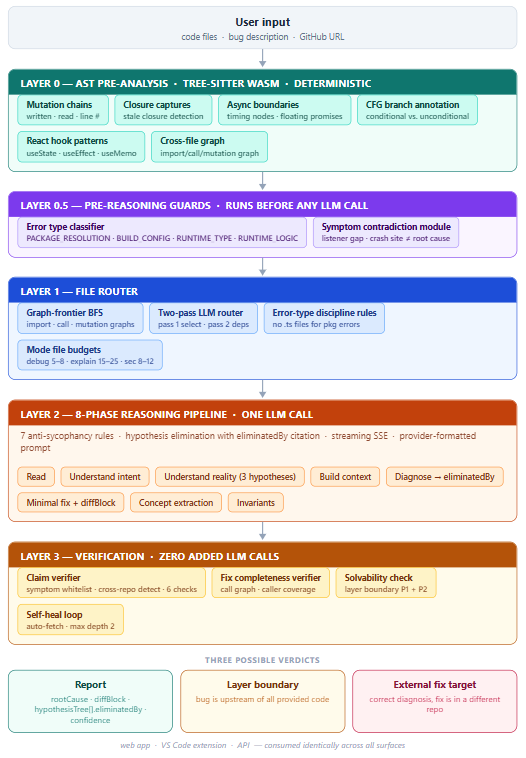
\includegraphics[width=0.92\linewidth]{1.png}
\caption{Unravel four-layer architecture. Layer~0.5 (Pre-Reasoning Guards) runs after
AST extraction and before the LLM call, injecting symptom contradiction alerts and
classifying the error type to govern downstream routing and verification behaviour.
Three structured verdicts are possible: a normal diagnosis report, \code{LAYER\_BOUNDARY}
(bug is upstream of all provided code), and \code{EXTERNAL\_FIX\_TARGET} (correct
diagnosis, fix lives in a different repository).}
\label{fig:architecture}
\end{figure}

% ─── 3.1 Layer 0 ─────────────────────────────────────────────────────────────
\subsection{Layer 0 — AST Pre-Analysis Engine}
\label{sec:layer0}

\begin{l0box}[title={Layer 0: Deterministic AST Pre-Analysis}]
\small
The engine (\code{ast-engine-ts.js}) uses web-tree-sitter in WebAssembly. An earlier
version used Babel as the AST engine; this failed on large TypeScript monorepos with
complex generic type syntax. The migration to tree-sitter provides partial-parse
resilience: files with syntax errors still yield valid structural facts. Explicit
\code{tree.delete()} calls after each operation prevent WASM memory leaks at
repository scale.
\end{l0box}

\vspace{6pt}
\textbf{Scope Resolver.} A complete scope map is built as a prerequisite for all
downstream analysis. Every binding (variables, parameters, destructured names, hoisted
functions) is recorded with its scope level and parent chain.

\textbf{\code{extractMutationChains(tree)}} walks every assignment expression, augmented
assignment, update expression, object property mutation, destructuring assignment, and rest
pattern. Each write and read is recorded with the enclosing function name (via upward parent
traversal) and line number:

\begin{lstlisting}[language={},style=code]
Variable Mutation Chains:
  duration
    written: pause()    L69
    written: setMode()  L86
    read:    tick()     L55
    read:    start()    L42
    read:    reset()    L79
\end{lstlisting}

\textbf{\code{trackClosureCaptures(tree)}} identifies the three-part profile of a stale
closure: referenced inside a function, defined in a parent scope, written anywhere in
that parent scope.

\textbf{\code{findTimingNodes(tree)}} maps every async boundary. Enumerated
APIs: \code{setTimeout}, \code{setInterval}, \code{clearInterval},
\code{requestAnimationFrame} (rAF), \code{fetch}, \code{.then()},
\code{.catch()}, \code{.finally()}, \code{addEventListener},
\code{removeEventListener}. Explicit enumeration prevents reasoning
about async code as if execution order matches source order.

\textbf{\code{detectFloatingPromises(tree)}} uses an \code{isAwaited(node)} guard.
Walking upward from an async call: if the traversal reaches an \code{await\_expression}
before an \code{expression\_statement}, the call is properly awaited. If it reaches
\code{expression\_statement} first, the promise is floating: the operation runs but its
result and any rejection are discarded.

\textbf{\code{detectReactPatterns(tree)}} identifies React anti-patterns that are
syntactically valid JavaScript but semantically incorrect in React's rendering model.
Three patterns are detected: \code{setState} inside a timer without the state variable
in the dependency array; \code{useEffect} with side effects but no cleanup return; missing
dependency array entries in \code{useMemo}/\code{useCallback}.

\textbf{\code{detectDirectStateMutations(tree)}} specifically targets direct mutation of
React state variables -- the primary cause of stale UI bugs where data changes in memory
but the component does not re-render. The detection runs in two phases. First,
\textit{identity extraction}: the engine queries all \code{useState} call expressions and
walks the \code{variable\_declarator} parent to extract the state variable identifier from
the array destructuring pattern (from \code{const [items, setItems] = useState([])},
it captures \code{"items"}). Second, \textit{conflict scanning}: for each tracked state
variable, the engine performs a method scan (checking every call expression whose object
matches the state variable against a set of known in-place mutating methods: \code{push},
\code{pop}, \code{splice}, \code{sort}, \code{reverse}, \code{shift}, \code{unshift},
\code{fill}, and \code{copyWithin}) and a property scan (checking every
\code{member\_expression} on the left-hand side of an assignment, such as
\code{items.user = value}).

When either scan fires, the engine emits a verified annotation:
\textit{``Direct state mutation: \code{items.push()} mutates state in-place -- React will
NOT re-render. Use \code{setItems([...items, newItem])} instead.''}
This converts a structurally invisible bug (valid JavaScript, wrong React semantics) into
an explicit verified fact in the ground-truth block, preventing the model from treating
the mutation as benign side-effectful code. LLMs reliably overlook \code{items.push(x)}
because it is syntactically unremarkable; the AST annotation makes the React semantic
violation explicit before any token is generated.

\textbf{\code{detectGlobalMutationBeforeAwait(tree)}} targets a race condition class
that is structurally invisible without cross-statement analysis: module-scope state
written immediately before an \code{await} in the same statement block. This pattern
creates a concurrent race window -- the \code{await} yields to the event loop, allowing
a concurrent call to overwrite the shared state before the first call resumes. The
detection runs in three passes: (1)~collect all \code{let}/\code{var} declarations at
module scope (not \code{const}); (2)~identify all functions that write those variables,
and scan import statements for setter-named imports matching
\code{/\^{}(set|clear|reset|init)[A-Z]/}; (3)~for each function's statement block,
walk top-level statements in order -- when a setter call is followed by an
\code{await\_expression} in the same block, emit a structured annotation naming the
write line, the await line, and the async gap it creates. The Ghost Tenant case study
(\S\ref{sec:superbug}) demonstrates this detector converting a 4/6 diagnosis
(correct class, missing yield-point) to 6/6 on an 8-file, 1,100-line codebase.

\textbf{Cross-file resolution (\code{ast-project.js}).} After per-file analysis, a
cross-file pass builds the module map, resolves symbol origins across import/export
boundaries, expands mutation chains across file boundaries, and emits risk signals for
cross-file mutation, async state races, and stale closures.

\textbf{Symptom Contradiction Module.}\label{sec:symptom-contradiction} Before any LLM call, a heuristic pass compares the
user's symptom description against AST evidence. Two checks run in debug mode:
\begin{itemize}
  \item \textbf{Listener Gap:} If the symptom contains phrases like ``not firing'' or
        ``event not triggered'' but AST confirms \code{addEventListener} is wired for the
        relevant event type, an alert is injected: the listener exists, the bug is in the
        handler logic, not the binding.
  \item \textbf{Crash Site $\neq$ Root Cause:} If the symptom names a specific function
        and AST shows that function makes \textit{no writes} (reads state only), it is
        flagged as the crash site rather than the root cause. The model is instructed to
        trace backward from it, not diagnose it directly.
\end{itemize}
Alerts are injected as \texttt{SYMPTOM CONTRADICTION ALERTS} into the ground truth block.
They never block analysis; they bias the model toward correct framing before token
generation begins.

The combined AST output is injected as a structured ground-truth block framed explicitly
as instructions the model is not permitted to contradict:

\begin{lstlisting}[language={},style=code]
VERIFIED GROUND TRUTH -- confirmed by static analysis.
Instructions: do not contradict any fact below.
==========================================================
Variable Mutation Chains:
  duration
    written: pause() L69    <- potential root cause
    read:    tick() L55, start() L42, reset() L79

Async Boundaries:
  setInterval -> tick() [L57]
  addEventListener("visibilitychange") -> handler() [L110]

Closure Captures:
  tick() captures: duration, remaining, interval
  STALE CANDIDATE: tick() reads duration from outer scope
\end{lstlisting}

% ─── 3.1b Layer 0.5 ──────────────────────────────────────────────────────────
\subsection{Layer 0.5 — Pre-Reasoning Guards}

\begin{defbox}[title={Layer 0.5: Pre-Reasoning Guards}]
\small
Two deterministic checks execute after AST extraction and before any LLM call.
Their purpose is to prevent the model from accepting a false premise as its
starting constraint. Neither check blocks analysis; both inject corrective alerts
into the ground truth block so the model is challenged \emph{before} its first
token is generated.
\end{defbox}

\vspace{6pt}
\textbf{Error Type Classifier.} A zero-LLM-cost regex classifier assigns every
analysis request to one of four categories: \code{PACKAGE\_RESOLUTION},
\code{BUILD\_CONFIG}, \code{RUNTIME\_TYPE}, or \code{RUNTIME\_LOGIC}. This
classification propagates to three downstream systems: (1)~Layer~1's Pass~2
discipline rules (e.g.\ \code{PACKAGE\_RESOLUTION} errors are explicitly prohibited
from requesting \texttt{.ts}/\texttt{.js} source files, since package resolution
bugs are never fixed in application source code); (2)~the solvability check in
Layer~3, which short-circuits the \code{LAYER\_BOUNDARY} classifier for
configuration-fixable error types; and (3)~the claim verifier, whose cross-repo
detection behaviour is conditioned on whether the error is structural or runtime.

\textbf{Symptom Contradiction Module.} Described in \S\ref{sec:symptom-contradiction}.
Two checks run in debug mode: the Listener Gap check (user says ``not firing'' but
AST confirms \code{addEventListener} is wired) and the Crash Site $\neq$ Root Cause
check (user names a function that makes no state writes). Alerts are injected as
\texttt{SYMPTOM CONTRADICTION ALERTS} into the ground truth block. The model is
explicitly instructed to investigate the contradiction before accepting the user's
framing at face value.

\clearpage
% ─── 3.2 Layer 1 ─────────────────────────────────────────────────────────────
\subsection{Layer 1 — File Router}

\begin{l1box}[title={Layer 1: File Router}]
\small
Unravel supports three input modes. For \textbf{paste/upload} mode, a graph-frontier BFS
router traverses import and call graph edges from symptom-adjacent files. For
\textbf{GitHub URL} mode, a dedicated two-pass fetch pipeline operates as follows.
\end{l1box}

\subsubsection{GitHub File-Fetch Pipeline}

When given a GitHub repository or issue URL, the following pipeline executes before any
AST analysis:

\vspace{8pt}

% ─── GITHUB PIPELINE DIAGRAM ─────────────────────────────────────────────────
\begin{figure}[H]
\centering
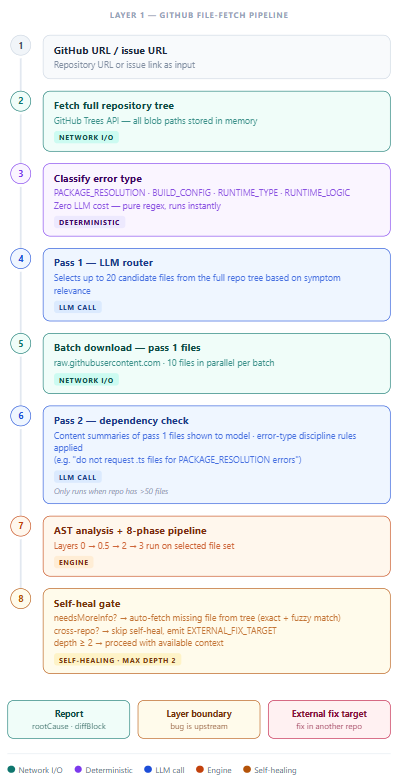
\includegraphics[width=0.72\linewidth,height=0.88\textheight,keepaspectratio]{2.png}
\caption{GitHub file-fetch pipeline (Layer~1). Step~3 classifies the error type
deterministically at zero LLM cost; this governs Pass~2 discipline rules (e.g.\
\code{PACKAGE\_RESOLUTION} errors are never routed to \texttt{.ts}/\texttt{.js}
source files). The self-heal gate distinguishes cross-repository references
(emits \code{EXTERNAL\_FIX\_TARGET}) from genuinely missing files (auto-fetches,
max depth~2).}
\label{fig:github}
\end{figure}

\textbf{Mode-specific file budgets} (upload/BFS mode):

\vspace{4pt}
\begin{center}
\begin{tabular}{@{}lcc@{}}
\toprule
\textbf{Mode} & \textbf{File Range} & \textbf{Selection Logic} \\
\midrule
Debug    & 5--8 files   & Max call-graph proximity to symptom \\
Explain  & 15--25 files & Breadth-first coverage \\
Security & 8--12 files  & Attack-surface paths \\
\bottomrule
\end{tabular}
\end{center}

\vspace{4pt}
Per-file truncation injects explicit \code{[TRUNCATED by Unravel]} markers. Every result
records \code{\_provenance.routerStrategy} (\code{"graph-frontier"}, \code{"llm-heuristic"},
or \code{"all-files"}), \code{engineVersion}, and \code{astVersion} for auditability.

% ─── 3.3 Layer 2 ─────────────────────────────────────────────────────────────
\subsection{Layer 2 — The 8-Phase Reasoning Pipeline}

\begin{l2box}[title={Layer 2: Core Engine}]
\small
One LLM call is made per analysis, but the system prompt enforces traversal through
eight phases in strict order. Phases~1--4 are shared across all three modes (Debug,
Explain, Security). Phases~5--8 are mode-specific. Phase~5 (DIAGNOSE) requires every
hypothesis elimination to populate \code{eliminatedBy} with the exact AST-verified
file and line that contradicts it; a hypothesis without a citation is flagged as
unverified reasoning. Phase~6 (MINIMAL FIX) produces a \code{diffBlock} field
containing a unified diff (\texttt{-- file:line / - old / + new}) in addition to
prose explanation.

Phase~6 defaults to the smallest possible surgical change. An \textit{architectural note}
is added -- never instead of the surgical fix, always in addition to it -- in any of
three cases: (A)~the patch suppresses the visible error but does not eliminate the
underlying incorrect state (a null-check around a crash site when null should never reach
there); (B)~the patch technically works but violates framework best practices or creates
maintenance debt (adding deps to a \code{useCallback} when the hook should be inlined
into \code{useEffect}; adding a lock around shared state when the real fix is to eliminate
shared ownership); or (C)~the bug exists because of wrong data ownership, shared mutable
state across async boundaries, or a missing abstraction layer that will cause the same
class of bug to recur. \code{RACE\_CONDITION} bugs involving shared async state
explicitly qualify for Case~C. The surgical patch remains actionable in all three cases;
the architectural note documents the structural property that was violated.

The prompt is formatted differently per provider: Claude receives
XML tags (\code{<instructions>}, \code{<rules>}, \code{<phase>}) for higher
instruction-following fidelity; Gemini receives Markdown headers; OpenAI-compatible
models receive section delimiters. The reasoning protocol is identical across providers.
\end{l2box}

\vspace{6pt}

% ─── 8-PHASE PIPELINE DIAGRAM ────────────────────────────────────────────────
\begin{figure}[H]
\centering
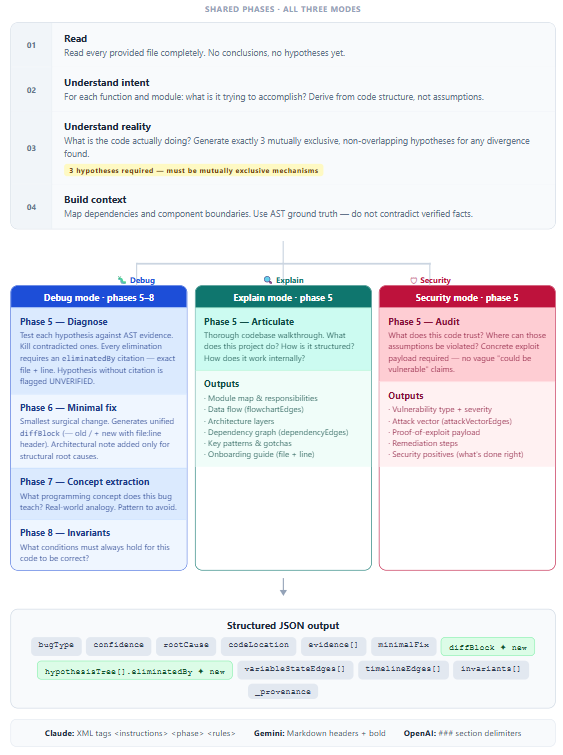
\includegraphics[width=0.92\linewidth]{3.png}
\caption{8-phase reasoning pipeline. Phases~1--4 are common to all three modes.
Phase~5 branches by mode; Debug mode continues through Phase~8. The
\code{eliminatedBy} field (new) requires each hypothesis elimination in Phase~5
to cite the exact AST-verified file and line that contradicts it; a hypothesis
without a citation is flagged as unverified reasoning. The \code{diffBlock} field
(new) in Phase~6 produces a unified diff (\texttt{-- file:line / - old / + new})
for every fix.}
\label{fig:pipeline}
\end{figure}

\textbf{Output schema.} Every analysis produces typed JSON consumed identically by the web
app, VS Code extension, and future clients. Beyond text fields, the schema includes graph
edge arrays (\code{timelineEdges}, \code{variableStateEdges}, \code{flowchartEdges},
\code{dependencyEdges}, \code{attackVectorEdges}) that the UI renders as interactive
\textbf{Mermaid diagrams}: a variable mutation flow graph, a multi-actor execution
sequence diagram with the bug point marked \code{isBugPoint: true}, and a data flow
flowchart. These visualizations are derived entirely from AST-verified structural facts,
not generated by the LLM.

\begin{lstlisting}[language=JSON, style=code]
{
  "bugType":      "STATE_MUTATION",
  "confidence":   0.92,
  "rootCause":    "Variable `duration` overwritten in pause() at line 69. All
                   subsequent reads in tick(), start(), reset() receive the
                   corrupted value.",
  "codeLocation": { "file": "script.js", "line": 69 },
  "evidence": [
    "AST confirms: duration written at pause() L69",
    "AST confirms: duration read at tick() L55 -- receives corrupted value"
  ],
  "diffBlock": "-- script.js L69\n-    duration = remaining\n+    lastActiveRemaining = remaining",
  "hypotheses": [
    { "id": "H1", "text": "Stale closure in tick() captures duration
                            at initialization",
      "status": "eliminated",
      "eliminatedBy": "script.js L55: tick() resolves duration from outer
                       scope at call time, not capture time",
      "reason": "Scope resolver confirms tick() resolves duration from
                 outer scope at call time, not capture time" },
    { "id": "H2", "text": "duration mutated in pause() before reset()",
      "status": "survived",
      "eliminatedBy": null,
      "reason": "Mutation chain confirms write at L69; reset() reads at L79" }
  ],
  "minimalFix": "Remove `duration = remaining` from pause(). duration must
                 remain constant for the session.",
  "invariants": ["duration must not change during active or paused session"],
  "_provenance": {
    "engineVersion": "3.3",
    "astVersion": "2.2",
    "routerStrategy": "graph-frontier",
    "model": "gemini-2.5-flash"
  }
}
\end{lstlisting}

\begin{figure}[H]
\centering
\includegraphics[width=\linewidth]{fig_mermaid.jpg}
\caption{Unravel renders two Mermaid-based visualizations from the structured JSON output.
\textit{Top:} Variable mutation flow graph -- edges show writes, reads, and cross-file
mutations for each tracked variable, with the causal path to the bug highlighted.
\textit{Bottom:} Multi-actor execution sequence diagram -- each actor is a function or
module; the \code{BUG HERE} marker is placed at the exact edge where the
\code{isBugPoint: true} flag is set in \code{timelineEdges}. Both diagrams are derived
from AST-verified structural facts, not generated by the LLM.}
\label{fig:mermaid}
\end{figure}

\begin{figure}[H]
\centering
\begin{minipage}[t]{0.54\linewidth}
  \includegraphics[width=\linewidth]{fig4a_webapp.jpg}
  \small\centering\textit{Web application: GitHub Import mode with Debug/Explain/Security\\modes and Quick Fix/Developer/Full Report presets.}
\end{minipage}
\hfill
\begin{minipage}[t]{0.43\linewidth}
  \includegraphics[width=\linewidth]{fig4b_vscode.jpg}
  \small\centering\textit{VS Code extension: right-click context menu exposing all three analysis modes directly in the editor.}
\end{minipage}
\caption{Unravel is consumed identically across surfaces. The web application is available
at \url{https://vibeunravel.netlify.app}. The VS Code extension is distributed as a
\code{.vsix} package installable via \textit{Extensions: Install from VSIX} in VS Code
(or \code{code --install-extension unravel.vsix} from the terminal), providing right-click
context menu access to all three modes on any open file. Both surfaces connect to the same
structured JSON pipeline; provider keys are stored locally and never transmitted.}
\label{fig:surfaces}
\end{figure}

\begin{figure}[H]
\centering
\includegraphics[width=0.88\linewidth]{fig_github.jpg}
\caption{Unravel GitHub repository
(\url{https://github.com/EruditeCoder108/unravelai}). The repository hosts the
web application source, the VS Code extension, the \code{ast-engine-ts.js} core,
the \code{orchestrate.js} pipeline, and the full UDB-20 benchmark suite under
\code{validation/}. License: BSL-1.1 (Business Source License -- converts to
open source after four years).}
\label{fig:github}
\end{figure}

% ─── 3.4 Layer 3 ─────────────────────────────────────────────────────────────
\subsection{Layer 3 — Verification and Integrity}

\begin{l3box}[title={Layer 3: Verification \& Integrity}]
\small
Four components execute synchronously after each LLM response, before any output is
surfaced. The Claim Verifier is the enforcement mechanism for the verified structural
facts injected in Layer~0: the LLM is not made infallible by prompt instruction, but
any output that contradicts injected facts is rejected deterministically here.
Three structured verdicts are possible: a normal diagnosis \textbf{Report}, a
\textbf{\code{LAYER\_BOUNDARY}} verdict when the root cause is upstream of all provided
code, and an \textbf{\code{EXTERNAL\_FIX\_TARGET}} verdict when the diagnosis is correct
but the fix must be applied in a different repository.
\end{l3box}

\vspace{6pt}
\textbf{Claim Verifier.} Six deterministic cross-checks against source files:
(1)~root cause file exists in provided inputs (hard rejection on failure);
(2)~cited line number is within file bounds;
(3)~evidence array filename references exist;
(4)~\code{codeLocation} file-line pairs validated via paired extraction;
(5)~security vulnerability file exists;
(6)~variable names in \code{evidence} present in the AST mutation map with fuzzy
matching for property access patterns. Violations above threshold set
\code{needsMoreInfo: true} and trigger the self-healing loop.

\textbf{Fix Completeness Verifier.} Uses the call graph from Layer~0 at zero additional
LLM calls and zero latency. For each function in \code{minimalFix}, all callers are
identified. If a caller file is absent from the fix, a warning is injected into the
\code{uncertainties} field and confidence is penalized by~0.15. React component files
(PascalCase filenames, \code{.jsx}/\code{.tsx} extensions) are excluded: fixing a custom
hook without modifying its consumers is encapsulation working as intended. The check fires
only on signature-breaking changes (removed parameters visible in \code{diffBlock}); backward-compatible
changes such as adding a guard or early return never trigger it, since callers require no
updates when the function's interface is unchanged.

\textbf{Claim Verifier precision improvements.} Five false-positive patterns were
identified and resolved across UDB-20 grading sessions. (1)~\textit{Class property
matching (B-05):} TypeScript class properties are stored in the AST as \code{this.propName};
the verifier now registers the bare name (\code{propName}) in addition to the prefixed
form so that AI-reported \code{currentConfig} correctly matches \code{this.currentConfig}.
(2)~\textit{Array subscript stripping (B-05):} variables reported as \code{serverLikeCounts[]}
are now normalized by stripping the bracket suffix before lookup.
(3)~\textit{Fix Completeness scope (B-05):} the completeness check previously fired on any
internal change; it now fires exclusively on diffs containing removed lines with function
parameter signatures -- backward-compatible additions (guards, early returns) do not
trigger it. (4)~\textit{Claim-side \code{this.} stripping (B-06):} the verifier
previously stripped \code{this.} only when building \code{knownVars}; it now also strips
it from the AI's claimed variable name at match time, so \code{this.isReady} in the
output correctly matches \code{isReady} in the AST. (5)~\textit{Empty-mutations skip
(B-07):} when \code{astRaw.mutations} is empty (no top-level variable mutations in the
scanned file set), Check~4 is skipped entirely -- previously, an empty \code{knownVars}
caused every claim to fail, generating false warnings on stable service registries.

\textbf{AST engine additions.} Four detection capabilities were added to
\code{ast-engine-ts.js} and are now active on all runs.

\textit{(1) \code{react\_unstable\_dep}:} Detects when a \code{useEffect} dependency
is created unstably inside a component body -- \code{new Service()}, \code{[]},
\code{\{\}}, or an arrow function -- without being wrapped in \code{useMemo} or
\code{useCallback}. This class of bug causes the effect to re-run on every render as
the object reference changes, accumulating subscriptions or side effects over time.

\textit{(2) \code{detectListenerParity()}:} Compares each \code{addEventListener} /
\code{removeEventListener} pair and emits a structured annotation. Mismatches in the
\code{capture} flag (which the DOM specification uses as part of listener identity) are
flagged as breaking. Mismatches in \code{passive} or \code{once} are flagged as
informational style warnings only, with the annotation explicitly stating:
\textit{``passive/once omission is harmless (spec: only capture affects identity).''}
This annotation directly prevented the pre-fix misdiagnosis on B-10 (\S\ref{sec:b10-two-runs}).

\textit{(3) \code{isWrappedInMemoHook()}:} Before flagging an object or function as
unstably created, the engine checks whether it is wrapped in \code{useMemo} or
\code{useCallback}. If it is, no instability flag is emitted. This prevents false
positives in codebases that correctly stabilize dependencies with memoization.

\textit{(4) \code{detectDirectStateMutations()}:} Targets direct in-place mutation of
React state variables -- the primary cause of stale UI bugs where data changes in memory
but the screen does not update. The detection uses two-phase identity-then-scan logic
described in \S\ref{sec:layer0}: state variable names are extracted from \code{useState}
destructuring, then each is checked against known in-place mutating methods (\code{push},
\code{splice}, \code{sort}, etc.) and direct property assignments. The emitted annotation
converts a structurally invisible bug (valid JavaScript, violated React rendering contract)
into an explicit verified fact: \textit{``Direct state mutation: \code{items.push()}
mutates state in-place -- React will NOT re-render.''} This completes Unravel's
React-specific pattern coverage: stale closures, missing dependencies, unstable
effect deps, listener lifecycle errors, and direct state mutation.

\textit{(5) \code{detectGlobalMutationBeforeAwait()}:} Detects module-scope state
written immediately before an \code{await} in the same statement block -- the
structural signature of a concurrent race window. The detector collects module-scope
writables, identifies setter functions and imported setters by naming convention
(\code{/\^{}(set|clear|reset|init)[A-Z]/}), then scans each function's statement
block for a setter-then-await adjacency, emitting a compound annotation naming the
exact write line, the exact yield line, and the async gap between them. This detector
is documented in detail in \S\ref{sec:superbug-detector}.

\subsection{Layer Boundary Detector}

\begin{defbox}[title={Definition: Layer Boundary Bug}]
\small
A \textit{layer boundary bug} is a defect whose causal origin resides in a software or
system layer outside the scope of the provided codebase. Attempting to fix such bugs from
within the application layer produces patches that are incorrect by construction: they
address a symptom of an upstream condition rather than the condition itself.
\end{defbox}

This insight arose from a concrete failure: when analyzing a VS Code keyboard issue where
\texttt{cmd+shift+]} failed on a Mac with the EurKEY layout, Unravel correctly traced the
root cause to the OS translating the physical \texttt{]} key into \texttt{Digit9} before
any VS Code code runs. Two completely different physical actions arrive looking identical at
the application boundary. The fix does not exist in the VS Code codebase, because the
distinguishing information was lost one layer upstream.

\textbf{Formal definition.} A diagnosis is classified as \code{LAYER\_BOUNDARY} when both
predicates hold:

\begin{lstlisting}[language={}, style=code]
P1 (deterministic):
  forall file_ref in extract_file_refs(rootCause):
    file_ref NOT IN provided_codebase
    AND NOT (verification.rootCauseRejected)   // hallucination != boundary

P2 (heuristic):
  exists keyword in UPSTREAM_KEYWORDS:
    keyword IN (rootCause OR evidence OR symptom)
\end{lstlisting}

P1 is the hard gate: if the root cause mentions any provided file, the check does not fire
regardless of keyword matches. P2 prevents false positives from bugs that simply omit file
names from the root cause text. The keyword set covers OS event routing, browser event
internals, Electron native bindings, external API layers, and keyboard layout translation.

\textbf{Confidence scoring.} The classifier assigns:
\[
  \text{confidence} = \min\!\bigl(0.95,\; 0.70 + 0.05 \times |\text{matched\_keywords}|
  + 0.10 \times \mathbf{1}[\text{rootCause cites no files}]\bigr)
\]

\textbf{Case study: tldraw CLI (PR~\#8161).} The primary CLI bug (wrong install directory)
was diagnosed as a \code{DATA\_FLOW} defect in the provided code. A secondary report
(files created after user cancellation) also triggered this detector: \code{ensureDirectoryEmpty}
calls \code{process.exit(1)} on cancellation, a behavior originating in npm's scaffolding
infrastructure upstream of the CLI code. Unravel correctly separated these two diagnoses
rather than generating a single incorrect fix.

\textbf{Self-Healing Context Loop.} Triggered by two signals detected after claim
verification: (A)~the model's \code{minimalFix} text contains phrases indicating it knows
the fix target is an unseen file (e.g.\ ``implementation is not provided''); or (B)~\code{codeLocation}
references a filename not present in the input set while the root cause cites a file that
is present. In GitHub URL mode, the missing file is automatically fetched from the stored
repository tree using exact path matching with fuzzy filename fallback. Depth is limited
to two iterations: the first reliably recovers direct missing dependencies; the second
resolves indirect imports discovered after the first fetch expands the visible interface
boundary. Beyond two iterations, additional file fetches expand context superlinearly while
rarely improving diagnostic resolution in practice.

\textbf{External Fix Target Verdict.} A third structured verdict (\code{EXTERNAL\_FIX\_TARGET})
is emitted when the claim verifier detects that the model's fix target belongs to an
external dependency package rather than the scanned codebase. This is distinguished from
hallucination by checking whether the cited file's package prefix matches a name present
in the project's dependency declarations. When triggered, the self-heal loop is skipped
entirely (the file is in a different repository and cannot be fetched from the local tree).
The full diagnosis is preserved alongside \code{targetRepository}, \code{targetFile},
and \code{suggestedAction} fields, giving the developer the complete root cause and a
precise pointer to where the fix must be applied.

\clearpage
% ─── 3.5 Output Presets and Diagnostic Invariants ───────────────────────────
\subsection{Output Presets and Diagnostic Invariants}

\textbf{Three analysis modes.} Unravel exposes three distinct analysis modes, each
sharing Phases~1--4 (Read, Understand Intent, Understand Reality, Build Context) before
branching at Phase~5:

\textit{Debug mode} (the primary mode) runs Phases~5--8: Diagnose, Minimal Fix,
Concept Extraction, and Invariants. It produces a structured diagnosis with root cause,
hypothesis tree with \code{eliminatedBy} citations, unified diff, and causal chain.
This is the mode used throughout UDB-20 and all case studies in this paper.

\textit{Explain mode} applies the same AST ground truth to produce a thorough codebase
walkthrough rather than a bug diagnosis. Output includes: entry point hierarchies
(file~+~line for every execution start), data flow graphs (\code{flowchartEdges}),
architecture layer groupings, component dependency maps (\code{dependencyEdges}),
non-obvious insights, and onboarding guides for common development tasks. The structural
analysis that makes debugging reliable -- knowing which functions call which, which
variables are shared, what the module graph looks like -- is precisely the knowledge that
makes onboarding expensive. Explain mode automates it deterministically.

\textit{Security mode} (beta) uses the call graph and mutation chains to trace data
from user-controlled inputs to sensitive operations. Each finding requires a concrete
exploit payload, a severity rating (Critical/High/Medium/Low/Informational), an
exploitability rating (Trivial/Moderate/Complex/Theoretical), and a confidence score.
Findings with confidence below~0.7 are automatically downgraded to Informational
regardless of stated severity. The mode also surfaces security positives -- things the
code does correctly -- to avoid the false impression that all findings are vulnerabilities.
Attack vector chains are rendered as \code{attackVectorEdges} for Mermaid flowcharts.

All three modes are available on the web application and VS Code extension and produce
the same structured JSON consumed identically across surfaces.

Unravel exposes three output presets (Quick Fix, Developer, Full Report) and a user
experience level selector (Beginner, Vibe Coder, Basic, Developer). A key design
constraint governs both: \textit{presets and levels control presentation, not diagnostic
depth.}

\textbf{Preset-invariant diagnostic core.} The 8-phase reasoning pipeline executes
identically across all presets. Critically, the output fields that enforce hypothesis
elimination -- \code{hypothesisTree}, \code{eliminatedBy}, \code{evidence[]},
\code{proximate\_crash\_site}, and \code{diffBlock} -- are bundled into the \code{rootCause}
schema group and cannot be removed by any preset. This is an architectural invariant:
a Quick Fix run and a Full Report run receive the same system prompt, the same 8-phase
reasoning instructions, and the same diagnostic output requirements. The only difference
is that Full Report additionally requests presentational sections (execution timeline,
concept extraction, invariants, variable state visualization). An engine that produces
a weaker root cause diagnosis under Quick Fix mode than Full Report mode is exhibiting
a prompt construction defect, not expected behavior. The UDB-20 mode parity policy
(\S\ref{sec:udb20}) explicitly grades for this.

\textbf{Level-scope constraint.} The user experience level (Beginner through Developer)
governs the \textit{explanation style} of text fields -- the warmth of the analogy,
the jargon density of \code{whyFixWorks}, the complexity of \code{conceptExtraction}.
It does not govern the diagnostic fields. The level instructions are explicitly prefixed
with a diagnostic precision mandate: evidence citations, line numbers, mutation chains,
and hypothesis eliminations are produced at full technical accuracy regardless of
audience. The model is instructed to \textit{do expert-level tracing first, then translate
the explanation} -- not to simplify the tracing itself. A beginner user receives the same
root cause, the same evidence, and the same fix as an intermediate developer; they receive
it explained differently.

\textbf{Language-scope constraint.} The output language selector (English, Hinglish, Hindi)
governs natural language production only. The English instruction was revised from
a simplification mandate (``explain like a 15-year-old'') to a professional neutral
baseline that inherits depth from the level instruction. Indian cultural analogies are
gated to Hinglish and Hindi settings and do not appear in English output.

% ─── 4. ANTI-SYCOPHANCY RULES ────────────────────────────────────────────────
\section{Anti-Sycophancy Rules}

Every LLM debugging tool defaults to agreement. If the symptom description names a
component, the model focuses on it. If a user proposes an incorrect hypothesis, supporting
evidence is generated rather than a contradiction~\cite{zhang2026}. Unravel embeds seven
rules hardcoded into every prompt: structural constraints on what the model is permitted to
output, not suggestions.

\begin{defbox}[title={Formal Failure Mode Definitions}]
\small
\textbf{Proximate Fixation:} The tendency of an LLM to attribute failure to the nearest
structurally familiar code to the crash or error site, rather than tracing state backward
to the distant origin of corruption. The model stops at the first plausible explanation
rather than eliminating alternatives.

\vspace{4pt}
\textbf{Name-Behavior Fallacy:} The tendency to assume that the semantic behavior of a
function or variable matches its identifier name, treating a function named \code{cleanup()}
as if it performs cleanup, or \code{isAuthenticated} as if it guarantees authentication,
without verifying the actual execution path.
\end{defbox}

\vspace{6pt}
\begin{center}
\rowcolors{2}{rowalt}{white}
\resizebox{\linewidth}{!}{%
\begin{tabular}{@{}c p{9.0cm} p{5.0cm}@{}}
\toprule
\textbf{\#} & \textbf{Constraint} & \textbf{Failure Mode Targeted} \\
\midrule
1 & If the code is correct, say ``No bug found.'' Do not invent defects. & Sycophantic RLHF alignment \\
2 & If the user's description contradicts the code, state the contradiction explicitly. & Confirmation bias \\
3 & If uncertain, say ``Cannot confirm without runtime execution.'' & Fabricated confidence \\
4 & Every bug claim requires an exact line number and code fragment. & Evidence fabrication \\
5 & Never describe code behavior not verifiable from the provided files. & Hallucinated behavior \\
6 & The crash site is the symptom. Trace state backward through mutation chains to where it was first corrupted. & Proximate Fixation \\
7 & A variable named \code{isPaused} does not guarantee the code pauses. Verify execution chains, not naming conventions. & Name-Behavior Fallacy \\
\bottomrule
\end{tabular}%
}
\end{center}

\vspace{6pt}
Rules~6 and~7 address the two most pervasive failure patterns identified in our analysis
of LLM debugging behavior. Rule~6 directly targets proximate fixation, the most cited
failure mode in the literature. Rule~7 targets a subtler failure: LLMs assign semantic
certainty to identifiers (\code{cleanup()}, \code{isAuthenticated}, \code{handleSave})
without verifying the actual execution path, missing bugs that look correct on a surface
reading precisely because they have semantically correct names.

% ─── 5. BUG TAXONOMY ─────────────────────────────────────────────────────────
\section{Bug Taxonomy}

Every diagnosis is classified against a 12-category formal taxonomy that is part of the
output schema. Classification enables cross-run pattern analysis and drives the concept
extraction phase.

\vspace{4pt}
\begin{center}
\rowcolors{2}{rowalt}{white}
\begin{tabular}{@{}l p{9.8cm}@{}}
\toprule
\textbf{Category} & \textbf{Description} \\
\midrule
\code{STATE\_MUTATION}   & Variable intended to be constant is modified unexpectedly \\
\code{STALE\_CLOSURE}    & Function captures outdated variable value \\
\code{RACE\_CONDITION}   & Multiple async operations conflict on shared state \\
\code{TEMPORAL\_LOGIC}   & Timing assumptions break: drift, wrong timestamps, sequence violations \\
\code{EVENT\_LIFECYCLE}  & Missing cleanup, double-binds, wrong event registration order \\
\code{TYPE\_COERCION}    & Implicit conversion causes unexpected computation \\
\code{ENV\_DEPENDENCY}   & Code behaves differently across environments \\
\code{ASYNC\_ORDERING}   & Operations execute in wrong sequence \\
\code{DATA\_FLOW}        & Data passes incorrectly between components or files \\
\code{UI\_LOGIC}         & Visual behavior does not match intended state \\
\code{MEMORY\_LEAK}      & Resources not released, accumulate over time \\
\code{INFINITE\_LOOP}    & Recursive or cyclic behavior creates runaway execution \\
\bottomrule
\end{tabular}
\end{center}

% ─── 6. EVALUATION ───────────────────────────────────────────────────────────
\section{Evaluation}

The primary quantitative evidence is \textbf{UDB-20}: a 20-bug reproducible benchmark
evaluated on three axes designed to directly measure the failure modes Unravel targets.
UDB-20 results (119/120 vs.\ 112/120) and the Ghost Tenant Super-Bug case study
are presented first. Real-world PR validation and comparative evaluation follow as
supplementary evidence. UDB-11 is retained as historical context only.

\textbf{Summary:} Unravel 125/126 (99.2\%) vs.~Claude~Sonnet~4.6 baseline 118/126
(93.7\%), delta $+$7. All Unravel experiments use Gemini~2.5~Flash -- a model priced
20$\times$ lower than the baseline (see model comparison, \S\ref{sec:udb20}).

\subsection{Evaluation Methodology}

\subsubsection{UDB-20 Three-Axis Rubric}
\label{sec:udb20}

UDB-20 scores each diagnosis on three independent axes, each scored 0--2, for a maximum
of 6 points per bug and 120 points across all 20 bugs. The three axes are designed to
independently measure the specific failure modes Unravel's architecture addresses.

\vspace{4pt}
\begin{center}
\rowcolors{2}{rowalt}{white}
\begin{tabular}{@{}l p{9.5cm}@{}}
\toprule
\textbf{Axis} & \textbf{Definition} \\
\midrule
\textbf{RCA} Root Cause Accuracy &
  2: Correct file + correct mechanism + correct lines (within ±3). \newline
  1: Correct file, wrong mechanism — or correct mechanism, wrong file. \newline
  0: Wrong file, wrong mechanism, or refusal to diagnose. \\
\textbf{PFR} Proximate Fixation Resistance &
  2: Explicitly names the planted trap and eliminates it with code evidence. \newline
  1: Finds correct root cause but never explicitly rebuts the trap. \newline
  0: Fixates on the trap or spends \textgreater50\% of diagnosis on the wrong location. \\
\textbf{CFR} Causal Flow Reconstruction &
  2: Full chain — root cause → intermediate state change → symptom, with file/line evidence at each hop. \newline
  1: Partial chain — missing intermediate steps, or no evidence for each hop. \newline
  0: No causal chain. States fix without explaining mechanism. \\
\bottomrule
\end{tabular}
\end{center}

\vspace{6pt}
The PFR axis is central to Unravel's thesis. Every bug in UDB-20 contains a \textit{planted
proximate trap}: a plausible-looking location that a naive model will fixate on, typically
the crash site or the file named in the symptom report. PFR measures whether the engine
explicitly eliminates the trap with evidence rather than passively arriving at the correct
location. An engine that always scores PFR~$=1$ (passively correct) is susceptible to
confident-wrong outputs on harder bugs where the correct location is less obvious.

The CFR axis captures a failure mode complementary to PFR: an engine can identify the
correct root cause file and mechanism, then fail to explain \textit{how} that cause produces
the observed symptom. A CFR~$=0$ answer is effectively unactionable -- the developer
cannot verify the diagnosis or trust the fix without independently retracing the causal chain.

\textbf{Hallucination penalty.} If an engine cites a line number that does not exist in
the provided files, or claims a variable appears at a location where it does not, the
entire axis in which that hallucinated evidence was used is capped at~0. This is the
structural HR rule: hallucinated evidence does not partially degrade a score, it
invalidates it.

\textbf{Mode parity policy.} All three output presets (Quick Fix, Developer, Full Report)
must produce equal RCA, PFR, and CFR quality. Mode differences are noted separately and
flagged as an engine defect, not a valid score variance. This policy reflects the design
principle that presets control \textit{output volume}, not \textit{diagnostic depth}: the
8-phase reasoning pipeline and hypothesis elimination run identically regardless of preset.

\textbf{Difficulty tiers.}

\begin{center}
\begin{tabular}{@{}lll@{}}
\toprule
\textbf{Tier} & \textbf{Bugs} & \textbf{Description} \\
\midrule
Easy   & B-01 to B-07 & Single-file root cause. Trap in same feature area. \\
Medium & B-08 to B-14 & Cross-file root cause. Trap is a different module. \\
Hard   & B-15 to B-20 & Multi-hop causal chain. Trap structurally similar to root cause. \\
\bottomrule
\end{tabular}
\end{center}

\textbf{Ground truth and verifiability.} Each bug in UDB-20 ships with:
(a)~\code{bug.test.*} -- a test that fails before the fix, confirming the bug is real;
(b)~\code{fixed.test.*} -- a test that passes after the ground truth fix, confirming the
fix is correct; (c)~\code{ground-truth.md} -- exact root cause file, lines, mechanism,
proximate trap, and correct fix. Ground truth is locked before any model sees the code.
Any researcher can independently run \code{pnpm test} to verify both the bug and the fix.
This is external validity by construction rather than author assertion.

\textbf{Grading.} All axes are graded by the author against \code{ground-truth.md}.
Results are archived in \code{validation/results/b-XX-<name>/grade.md} alongside raw
engine outputs. The full 3-axis rubric and scoring policies are published in
\code{validation/grading/README.md}.

\textbf{Implementation note: Model asymmetry.} All Unravel experiments were conducted
using \textbf{Gemini~2.5~Flash} (thinking mode, preview 04-17), a cost-optimised model
released approximately 11 months before this writing, designed for speed and
cost-effectiveness rather than peak capability. The baseline is
\textbf{Claude~Sonnet~4.6}, Anthropic's state-of-the-art model released in 2025,
purpose-built for coding and reasoning tasks and among the highest-scoring models on
real-world software engineering benchmarks. These are not comparable models.

\vspace{4pt}
\begin{table}[H]
\centering\small
\setlength{\tabcolsep}{4pt}
\begin{tabular}{@{}l p{3.2cm} cc@{}}
\toprule
\textbf{Benchmark} & \textbf{Domain} & \textbf{Gemini 2.5 Flash} & \textbf{Claude Sonnet 4.6} \\
\midrule
\multicolumn{4}{@{}l}{\textit{Reasoning \& knowledge}} \\
Humanity's Last Exam    & Broad reasoning        & 12.1\%  & 33.2\% \\
GPQA Diamond            & Graduate science       & 78.3\%  & 89.9\% \\
ARC-AGI-2               & Novel problem-solving  & --      & 58.3\% \\
\midrule
\multicolumn{4}{@{}l}{\textit{Coding}} \\
SWE-bench Verified      & Real-world GitHub bugs & --      & 79.6\% \\
LiveCodeBench v5        & Code generation        & 63.5\%  & -- \\
\midrule
\multicolumn{4}{@{}l}{\textit{Mathematics}} \\
AIME 2025               & Competition math       & 78.0\%  & -- \\
AIME 2024               & Competition math       & 88.0\%  & -- \\
\midrule
\multicolumn{4}{@{}l}{\textit{Pricing (at time of writing)}} \\
Input / 1M tokens  &  & \$0.15  & \$3.00 \\
Output / 1M tokens &  & \$0.60  & \$15.00 \\
\bottomrule
\end{tabular}
\caption{Published benchmark scores for the two models used in this evaluation.
Sources: Google AI Studio benchmark release (Gemini~2.5~Flash); Anthropic model card
(Claude~Sonnet~4.6). Dashes indicate the benchmark was not reported by that provider.}
\label{tab:model-comparison}
\end{table}

\vspace{4pt}
On every overlapping benchmark, Claude~Sonnet~4.6 leads substantially: Humanity's Last
Exam (33.2\% vs 12.1\%), GPQA Diamond (89.9\% vs 78.3\%). Its SWE-bench Verified score
of 79.6\% is one of the highest published on that benchmark -- which measures resolution
of real GitHub issues, exactly the task Unravel addresses. The input price differential
is 20$\times$.

This asymmetry is intentional and is itself a result. The thesis is that structural
pre-analysis compensates for model capability on multi-file bug diagnosis: the AST layer
delivers verified structural facts that the stronger model would otherwise find through
deeper reasoning. The Super-Bug result (\S\ref{sec:superbug}) makes this concrete --
Gemini~2.5~Flash with a 150-line targeted detector matched Claude~Sonnet~4.6 on an
extreme-difficulty race condition spanning 8 files and 1,100 lines. The structural
knowledge did the work that model scale would otherwise need to do.

\textbf{Additional metric definition.}
\begin{itemize}
  \item \textbf{Hallucination Rate (HR):} Percentage of diagnostic entity claims
        (file names, line numbers, variable names in the evidence block) that reference
        entities not present in the provided source files, as detected by the Claim
        Verifier's six deterministic checks.
        Formally: $\text{HR} = |\text{failed Claim Verifier checks}| /
        |\text{total entity claims assessed}|$.
\end{itemize}

\begin{findingbox}
\textit{Scope note.} HR measures \textbf{structured entity hallucination} only: fabricated
file names, line numbers, and variable references in the output schema. It does not capture
reasoning hallucination (confabulated causal chains) or behavioral hallucination
(unverifiable semantic claims). These remain open problems addressed by the proposed
Reasoning Integrity metric (\S\ref{sec:ri}).
\end{findingbox}

\subsubsection{Baseline Prompt Design and the Prompt Parity Question}
\label{sec:prompt-parity}

A methodological revision was made at B-12 that affects how the baseline results for
B-12 onward should be interpreted. We document it here in full because it strengthens
the benchmark's validity rather than weakening it.

\textbf{The original baseline (B-01--B-11).} The baseline for the first eleven bugs was
Claude~Sonnet~4.6 with a minimal prompt: the source files and the \code{symptom.md}
report, with no instruction on output format or reasoning structure. This is the prompt
that most developers use when asking a model to debug their code -- a realistic baseline
for how these tools are actually deployed. Unravel, by contrast, runs an 8-phase
structured pipeline that forces hypothesis generation, evidence-based elimination, and a
causal chain at every step, with a JSON schema that requires these fields be populated.
The resulting outputs are structurally asymmetric.

During grading of B-01--B-11, the CFR gap (Unravel 20/20, baseline 14/20) was examined
and found to be partially attributable to this asymmetry. The baseline was not failing to
\textit{reason} about causal chains; it was failing to \textit{produce} them, because no
instruction asked for them. Scoring a model on a dimension it was never asked to produce
measures output format compliance, not diagnostic capability. The RCA and PFR scores
remain valid -- both engines received identical symptom reports and both were asked to
identify the root cause -- but the CFR scores for B-01--B-11 carry a format-artifact
caveat that is acknowledged explicitly in the results.

\textbf{The structured baseline (B-12 onward).} Starting from B-12, the baseline prompt
was revised to match the structural requirements Unravel imposes on itself. The prompt
instructs the model to: list three candidate hypotheses and state whether each is
ELIMINATED or SURVIVED with exact file and line citation; state the root cause with
exact file, line, and mechanism; trace the full causal chain with file and line at every
hop; explicitly name the proximate trap and state why it is not the root cause with
evidence; and provide the minimal fix. With this prompt, Claude~Sonnet~4.6 scored 6/6
on B-12. This is the expected result on a medium-difficulty data flow bug with a linear
causal chain -- a capable model with explicit chain-tracing instructions should find it.
The tie on tractable bugs is not a failure of the benchmark; it is the correct baseline
behavior. Where the AST advantage should emerge is on bugs where reading alone is
insufficient.

\textbf{Is Unravel just a better prompt?} This question deserves a direct answer.

When Claude produces a hypothesis tree under the structured prompt, the file names, line
numbers, and causal facts come from \textit{probabilistic inference over the source text}:
the model reads the code and pattern-matches to the most plausible chain. When Unravel
produces a hypothesis tree, the structural facts were \textit{deterministically extracted
before the model ran}: the exact lines where every variable is mutated, the precise set
of event listeners registered vs.\ removed, whether each mutation is branch-gated or
unconditional. The model does not infer these; it reads them from a verified fact table.

The practical difference is visible in B-10. Claude with the structured prompt scored
4/6: it correctly dismissed the \code{passive} options mismatch and correctly
hypothesized concurrent mounted instances as the mechanism, but could not confirm the
hypothesis from the provided files and flagged its diagnosis as inconclusive -- correct
reasoning, bounded by available context. Unravel without the AST fix also scored 4/6,
for the opposite reason: it anchored on the \code{passive} mismatch because no
authoritative counter-fact was available. After \code{detectListenerParity()} added
47 words of verified DOM spec annotation, Unravel scored 6/6. The change was not a
better prompt and not a more capable model. It was a \textit{deterministic fact} that
no amount of careful code-reading could have reliably produced.

Verified structural knowledge does not make the model smarter. It eliminates entire
categories of false hypothesis before they can form. On bugs where careful reading is
sufficient, a structured prompt and AST grounding will produce identical results. On
bugs where the relevant fact is non-obvious, spans more context than the model can hold,
or requires domain knowledge embedded in a spec, only the deterministic layer provides
the necessary constraint. The B-12--B-20 harder bugs and the final large-codebase case
study are designed to test exactly this boundary. Using the structured prompt from B-12
onward makes any remaining delta attributable to the AST contribution, not the output
format -- which is a stronger and more honest result.


% ─── 6.2 UDB-20 Results ──────────────────────────────────────────────────────
\subsection{UDB-20 Results (B-01 to B-20)}
\label{sec:udb20-results}

All 20 bugs have been constructed, run, and graded against locked ground truth.
The baseline for B-01--B-11 is Claude~Sonnet~4.6 with a minimal prompt (the
symptom report and source files only -- the realistic baseline for how these tools
are deployed). From B-12 onward, the baseline uses the structured prompt described
in \S\ref{sec:prompt-parity}. B-10 was run twice: both scores are reported
(\S\ref{sec:b10-two-runs}). The Super-Bug case study is reported separately
(\S\ref{sec:superbug}).

\vspace{6pt}
\begin{table}[H]
\centering\small
\setlength{\tabcolsep}{3pt}
\resizebox{\linewidth}{!}{%
\begin{tabular}{@{}l l l *{3}{c} c @{\hspace{3pt}} *{3}{c} c@{}}
\toprule
& & & \multicolumn{4}{c}{\textbf{Unravel (Gemini~2.5 Flash + AST)}}
    & \multicolumn{4}{c}{\textbf{Baseline (Claude~Sonnet~4.6)}} \\
\cmidrule(lr){4-7}\cmidrule(lr){8-11}
\textbf{Bug} & \textbf{Tier} & \textbf{Category}
  & \textbf{RCA} & \textbf{PFR} & \textbf{CFR} & \textbf{/6}
  & \textbf{RCA} & \textbf{PFR} & \textbf{CFR} & \textbf{/6} \\
\midrule
\multicolumn{11}{@{}l}{\textit{\small B-01--B-11: baseline used unstructured prompt}} \\
B-01 \textit{invisible-update}    & Easy   & STATE\_MUTATION    & 2 & 2 & 2 & \textbf{6} & 2 & 2 & 1 & 5 \\
B-02 \textit{phantom-preference}  & Hard   & STATE\_MUTATION    & 2 & 2 & 2 & \textbf{6} & 2 & 2 & 1 & 5 \\
B-03 \textit{loyal-closure}       & Medium & STALE\_CLOSURE     & 2 & 2 & 2 & \textbf{6} & 2 & 2 & 1 & 5 \\
B-04 \textit{deaf-plugin}         & Hard   & STALE\_CLOSURE     & 2 & 2 & 2 & \textbf{6} & 2 & 2 & 1 & 5 \\
B-05 \textit{fickle-like}         & Medium & ASYNC\_ORDERING    & 1 & 2 & 2 & 5          & 2 & 2 & 1 & 5 \\
B-06 \textit{silent-await}        & Easy   & ASYNC\_ORDERING    & 2 & 2 & 2 & \textbf{6} & 2 & 1 & 2 & 5 \\
B-07 \textit{ghost-ref}           & Medium & ASYNC\_ORDERING    & 2 & 2 & 2 & \textbf{6} & 2 & 2 & 2 & \textbf{6} \\
B-08 \textit{twin-effect}         & Medium & EVENT\_LIFECYCLE   & 2 & 2 & 2 & \textbf{6} & 2 & 2 & 2 & \textbf{6} \\
B-09 \textit{trusted-input}       & Hard   & TYPE\_COERCION     & 2 & 2 & 2 & \textbf{6} & 2 & 2 & 2 & \textbf{6} \\
B-10 \textit{orphan-listener}     & Hard   & EVENT\_LIFECYCLE   & 2 & 2 & 2 & \textbf{6}$^\dagger$ & 1 & 2 & 1 & 4 \\
B-11 \textit{dropped-field}       & Medium & DATA\_FLOW         & 2 & 2 & 2 & \textbf{6} & 2 & 2 & 1 & 5 \\
\midrule
\multicolumn{11}{@{}l}{\textit{\small B-12--B-20: baseline used structured prompt (\S\ref{sec:prompt-parity})}} \\
B-12 \textit{invisible-inventory} & Medium & DATA\_FLOW         & 2 & 2 & 2 & \textbf{6} & 2 & 2 & 2 & \textbf{6} \\
B-13 \textit{millisecond-session} & Medium & TEMPORAL\_LOGIC    & 2 & 2 & 2 & \textbf{6} & 2 & 2 & 2 & \textbf{6} \\
B-14 \textit{shared-window}       & Medium & DATA\_FLOW         & 2 & 2 & 2 & \textbf{6} & 2 & 2 & 2 & \textbf{6} \\
B-15 \textit{bootstrap-deadlock}  & Hard   & ASYNC\_ORDERING    & 2 & 2 & 2 & \textbf{6} & 2 & 2 & 2 & \textbf{6} \\
B-16 \textit{esm-shadow}          & Hard   & ENV\_DEPENDENCY    & 2 & 2 & 2 & \textbf{6} & 2 & 2 & 2 & \textbf{6} \\
B-17 \textit{unstable-config}     & Hard   & DATA\_FLOW         & 2 & 2 & 2 & \textbf{6} & 2 & 2 & 2 & \textbf{6} \\
B-18 \textit{lost-increment}      & Hard   & RACE\_CONDITION    & 2 & 2 & 2 & \textbf{6} & 2 & 2 & 2 & \textbf{6} \\
B-19 \textit{phantom-gate}        & Hard   & ENV\_DEPENDENCY    & 2 & 2 & 2 & \textbf{6} & 2 & 2 & 2 & \textbf{6} \\
B-20 \textit{locked-key}          & Hard   & ENV\_DEPENDENCY    & 2 & 2 & 2 & \textbf{6} & 2 & 2 & 2 & \textbf{6} \\
\midrule
\textbf{Total /120} & & & \textbf{39} & \textbf{40} & \textbf{40} & \textbf{119}
                          & 39 & 39 & 34 & \textbf{112} \\
\bottomrule
\end{tabular}%
}
\vspace{2pt}
{\small $^\dagger$B-10 post-fix score. Pre-fix: 4/6. Both runs in \S\ref{sec:b10-two-runs}.}
\caption{UDB-20 complete results. RCA, PFR, CFR each 0--2; per-bug max~6, full benchmark max~120.
Unravel: 119/120 (99.2\%). Baseline: 112/120 (93.3\%). Delta: $+$7.
B-01--B-11 baseline: unstructured prompt. B-12--B-20 baseline: structured prompt (\S\ref{sec:prompt-parity}).}
\label{tab:udb20}
\end{table}

\vspace{6pt}
\begin{table}[H]
\centering\small
\resizebox{\linewidth}{!}{%
\begin{tabular}{@{}l ccc c p{8.5cm}@{}}
\toprule
\textbf{Axis} & \textbf{Unravel /40} & \textbf{Baseline /40} & \textbf{$\Delta$} & \textbf{Pattern} \\
\midrule
RCA & 39 & 39 & 0   & Tied overall. B-05 Unravel wrong file; B-10 baseline wrong mechanism. \\
PFR & 40 & 39 & $+$1 & B-06 baseline half-credit (trap acknowledged, not eliminated). \\
CFR & 40 & 34 & $+$6 & Full chains on all 20. Baseline dropped hops on B-01--B-05, B-10--B-11. \\
\midrule
\textbf{Total} & \textbf{119} & \textbf{112} & $\mathbf{+7}$ & \\
\bottomrule
\end{tabular}%
}
\caption{Per-axis aggregate across all 20 bugs. The entire +7 gap is from B-01--B-11
(unstructured baseline). With structured prompt (B-12--B-20): Claude 54/54 (100\%),
Unravel 53/54 (98.1\%). B-10 is the only structured-prompt gap and required a
DOM spec annotation to resolve (\S\ref{sec:b10-two-runs}).}
\label{tab:udb20-axes}
\end{table}

\begin{findingbox}
\textbf{Key findings from B-01--B-20.}

\textbf{CFR is the dominant differentiator in the unstructured era.} Unravel scored
CFR~$=2$ on all 20 bugs (40/40). In the unstructured baseline era (B-01--B-11), the
baseline scored CFR~$=1$ on 7 of 11 bugs -- dropping hops on every multi-file chain.
With the structured prompt (B-12--B-20), the baseline scored 20/20 on CFR. As discussed
in \S\ref{sec:prompt-parity}, the B-01--B-11 CFR gap partially reflects output format
rather than pure reasoning capability; the structured prompt closes it on tractable bugs.

\textbf{The structured prompt era (B-12--B-20): near-identical performance.}
With the structured prompt, Claude~Sonnet~4.6 scored 54/54 (100\%) on B-12--B-20.
Unravel scored 53/54 (98.1\%), the single dropped point being B-05's wrong-file
diagnosis from the earlier unstructured era. On the nine bugs run with the structured
prompt, every score was a tie at 6/6. This is the expected result: on medium and hard
bugs with linear or moderately complex causal chains, a capable model with the right
output structure matches deterministic AST grounding.

\textbf{B-10 and B-16 show the difference between deterministic extraction and reading.}
Both engines produced correct diagnoses on B-16 (\textit{esm-shadow}), but by
different mechanisms. Unravel's AST engine produced a \code{variableStateEdges} graph
that deterministically tracked \code{\_\_dirname} as defined in \code{app.ts} scope and
undefined in \code{pathUtils.ts} scope -- a structural cross-file fact. The baseline
read both files and applied training-data knowledge of ESM scoping rules to infer the
same conclusion. The result is identical; the provenance is not. B-10 shows what happens
when the two diverge: the \code{passive} listener identity rule is an obscure DOM spec
edge case. The baseline's training data produced the wrong answer (passive mismatch
breaks removal). The AST annotation provided the correct spec fact as verified ground
truth, and the wrong answer did not occur.

\textbf{B-05 is the only Unravel failure.} Correct mechanism, wrong file.
Caller-side guard placement required design-intent reasoning not visible in the AST.
The remaining 19/20 bugs were perfect.
\end{findingbox}

\subsubsection{B-10: Two Runs and What One AST Annotation Changed}
\label{sec:b10-two-runs}

B-10 (\textit{orphan-listener}) is the only bug where the AST engine was modified
between runs. Both runs are reported; only the post-fix score appears in the aggregate.

\textbf{Pre-fix run (Unravel 4/6, Baseline 4/6).} The ground truth root cause is
accumulated scroll listeners from \code{PageView} components not being properly unmounted
during SPA navigation. Unravel (pre-fix) identified the correct file but anchored on the
syntactic asymmetry between \code{addEventListener('scroll', fn, \{passive:\ true\})} and
\code{removeEventListener('scroll', fn)} (no options object). Per the DOM specification,
\code{passive} is not part of the listener identity key for removal; only \code{capture}
is. The proposed fix was a no-op. The baseline also scored 4/6 but for different reasons:
it correctly dismissed the \code{passive} mismatch, correctly hypothesized concurrent
mounted instances as the mechanism, but could not confirm the hypothesis from the three
provided files. Correct reasoning, insufficient context.

\textbf{Post-fix run (Unravel 6/6).} \code{detectListenerParity()} was added to
\code{ast-engine-ts.js}. When options differ only in \code{passive} or \code{once}, the
annotation states: \textit{``passive/once omission is harmless (spec: only capture affects
identity).''} This 47-word annotation appears in the verified ground-truth block before the
LLM sees the code. Hypothesis~H1 (\code{passive} mismatch) was eliminated immediately in
Phase~5, citing the annotation verbatim. Hypothesis~H3 (multiple \code{PageView} instances
not unmounting) survived and was confirmed. The LLM did not hallucinate about
\code{passive} because it was careless -- it hallucinated because no authoritative
counter-fact was available. Once the AST provided the counter-fact as verified ground
truth, the hallucination did not occur.


% ─── 6.3 Super-Bug Case Study ────────────────────────────────────────────────
\subsection{Case Study: Ghost Tenant -- A Race Condition Across 8 Files}
\label{sec:superbug}

To probe the boundary between what careful reading can produce versus what requires
verified structural analysis, we evaluated Unravel and the structured-prompt baseline
on a constructed extreme-difficulty bug: a multi-tenant data isolation failure in a
production-scale SaaS API. The same codebase, the same symptom description, and the
same underlying model (Gemini~2.5~Flash) were evaluated twice -- once with the
pre-existing AST engine, and once after adding a targeted detector. The results
constitute a controlled experiment on what deterministic structural extraction adds
over reading alone on a bug with 1,100 lines of surface noise.

\textbf{The bug.} Category: \code{RACE\_CONDITION} + \code{STATE\_MUTATION}.
Setting: a multi-tenant document API serving enterprise customers. Under concurrent
production load ($\sim$2,000 req/min), documents belonging to Tenant~B appear in
Tenant~A's API responses with a failure rate of approximately 1 in 300 requests --
invisible in development, data-isolation-breaking in production.

The root cause is two adjacent lines in \code{TenantMiddleware.ts}:
\begin{lstlisting}[language=JavaScript,style=code]
setTenant(req.tenantId);                // L75 -- writes module-level _activeTenant
await verifyTenantExists(req.tenantId); // L76 -- async gap opens here (~20ms)
\end{lstlisting}
\code{\_activeTenant} is declared at module scope in \code{TenantContext.ts} -- a single
shared variable for the entire Node.js process. The \code{await} at L76 suspends
execution and yields to the event loop. Any concurrent request arriving during this
$\sim$20ms window calls \code{setTenant()} with its own tenant ID, overwriting
\code{\_activeTenant}. Every downstream operation -- cache key construction, SQL WHERE
clause parameterisation, audit log entries -- reads the poisoned global. The minimal
fix is a two-line swap: await first, then set. The architectural fix is
\code{AsyncLocalStorage}, which provides per-request isolated storage propagating
automatically across \code{await} boundaries.

\textbf{The three planted traps.} The symptom description aggressively directed attention
at three structurally plausible but incorrect locations. (H1)~\code{TenantCache.ts}:
\code{buildKey()} uses \code{getTenant()} and the cache key logs show the wrong tenant
ID -- correct observation, wrong conclusion. The cache is a consumer of a corrupt value,
not its producer; the AST call graph confirms \code{TenantCache.ts} has zero writes to
\code{\_activeTenant}. (H2)~\code{AuthMiddleware.ts}: if JWT extraction produced the
wrong tenant, all downstream operations would be wrong. Eliminated by the call graph:
\code{AuthMiddleware.ts} has zero imports of \code{TenantContext} and zero reads or
writes of \code{\_activeTenant}. (H3)~\code{QueryBuilder}'s WHERE clause: uses
\code{getTenant()} -- correct observation. The WHERE clause logic is correct; the
parameter it receives is corrupt before it arrives. None of these can be eliminated
by reading the files sequentially; each requires a cross-file structural fact about
which functions write to \code{\_activeTenant}.

\subsubsection{Run 1: Without the Targeted Detector (Unravel 4/6)}
\label{sec:superbug-run1}

\textbf{Inputs:} 8 source files, symptom description, Gemini~2.5~Flash, full Unravel
pipeline with the pre-existing AST engine.

The existing engine surfaced \code{\_activeTenant} in the mutation chain as a
module-scope variable with writes in \code{setTenant()} and \code{clearTenant()}, and
the cross-file call graph showing \code{getTenant()} called in \code{QueryBuilder.ts},
\code{TenantCache.ts}, and \code{AuditLogger.ts}. What it did not produce was a compound
signal connecting the write in \code{TenantMiddleware.ts} to the adjacent \code{await}
in the same statement block -- the precise relationship that defines the race window.

\begin{center}\small
\begin{tabular}{@{}lcc@{}}
\toprule
\textbf{Axis} & \textbf{Score} & \textbf{Notes} \\
\midrule
RCA & 1/2 & Correct global as shared state; missed the L75--L76 yield-point mechanism \\
PFR & 2/2 & Eliminated TenantCache (downstream), AuthMiddleware (no context writes) \\
CFR & 1/2 & Generic: "Request A sets tenant, Request B overwrites it" -- no await hop \\
\midrule
\textbf{Total} & \textbf{4/6} & Proposed AsyncLocalStorage but not the two-line swap \\
\bottomrule
\end{tabular}
\end{center}

For a 1,100-line codebase, identifying the exact write-before-await compound relationship
across 8 files exceeded the reliable inference threshold of Gemini~2.5~Flash. The model
knew the global was dangerous but did not identify the specific 20ms yield window.

\subsubsection{Targeted Detector: \code{detectGlobalMutationBeforeAwait()}}
\label{sec:superbug-detector}

The gap was precise and fixable. A 150-line detector was added to \code{ast-engine-ts.js}
running in three passes. \textit{Pass A -- module-scope writables:} walks direct children
of the root node, collects all \code{let} and \code{var} declarations at module scope
(not \code{const} -- immutable bindings cannot be reassigned across requests). In
\code{TenantContext.ts}, this finds \code{\_activeTenant}. \textit{Pass A -- setter
discovery:} finds every function whose body contains an assignment to a collected
module-scope variable (\code{setTenant}, \code{clearTenant}), and scans import statements
for identifiers matching the pattern \code{/\^{}(?:set|clear|reset|init)[A-Z]/} to catch
imported setters. \textit{Main scan:} for each function's statement block, walks
top-level statements in order. When a statement is a call to a recognised setter, looks
at subsequent statements for the first \code{await\_expression}. On match, emits:
\begin{lstlisting}[language={},style=code]
Global State Written Before Async Yield  CONCURRENT RACE RISK:
  setTenant [TenantMiddleware.ts] written at L75  then await at L76  in `handle`
  During the async gap, any concurrent call to `handle` will overwrite this value.
  All code reading this global after the await may receive a different caller's state.
  Fix: move the write to AFTER the await resolves, or use AsyncLocalStorage.
\end{lstlisting}
This signal is injected as verified ground truth -- the same status as mutation chains.
The model cannot contradict it, cannot attribute a different line number to the write.

\subsubsection{Run 2: With the Targeted Detector (Unravel 6/6)}
\label{sec:superbug-run2}

\textbf{Inputs:} Identical to Run~1. Only change: \code{detectGlobalMutationBeforeAwait()} now runs.

\begin{center}\small
\begin{tabular}{@{}lcc@{}}
\toprule
\textbf{Axis} & \textbf{Score} & \textbf{Notes} \\
\midrule
RCA & 2/2 & Exact: \code{TenantMiddleware.ts L75-L76} + \code{TenantContext.ts L1} \\
PFR & 2/2 & All three traps eliminated with file+line evidence \\
CFR & 2/2 & 9-hop timeline including exact concurrent interleaving and yield point \\
\midrule
\textbf{Total} & \textbf{6/6} & \\
\bottomrule
\end{tabular}
\end{center}

The \code{rootCause} field from Run~2: \textit{``Race condition on shared mutable
module-level state (\code{\_activeTenant} in \code{TenantContext.ts}) where
\code{TenantMiddleware.handle} (L75) writes the tenant ID before an \code{await} (L76),
allowing a concurrent request to overwrite the state before the first request resumes.''}
The yield point is named. The specific lines are cited. The \code{evidence} field
explicitly cited the AST signal as its source: \textit{``VERIFIED STATIC ANALYSIS:
Global State Written Before Async Yield -- \code{setTenant} written at L75, then
\code{await} at L76 in \code{handle}.''} The model cited the AST signal as evidence.
This is the expected behavior: the detector produces a fact; the model uses the fact;
the fact appears in the output with its provenance.

\subsubsection{Baseline Performance (Claude Sonnet 4.6, Structured Prompt: 6/6)}
\label{sec:superbug-claude}

Claude~Sonnet~4.6 with the structured prompt scored 6/6 on the Super-Bug on its
first run, with no AST context. It identified both the shared global (\code{TenantContext.ts:1})
and the exact yield point (\code{TenantMiddleware.ts:62-63}), producing the complete
9-hop timeline and explicitly dismantling the \code{TenantCache.ts} trap with the
observation that the cache, query builder, and audit logger are all victims: fixing the
cache would mask the symptom for one call site while \code{QueryBuilder} and
\code{AuditLogger} would still read the poisoned global.

\begin{center}\small
\begin{tabular}{@{}l cc@{}}
\toprule
& \textbf{Unravel Run 1} & \textbf{Unravel Run 2} \\
\midrule
RCA & 1/2 & 2/2 \\
PFR & 2/2 & 2/2 \\
CFR & 1/2 & 2/2 \\
\textbf{Total} & \textbf{4/6} & \textbf{6/6} \\
\bottomrule
\end{tabular}
\quad
\begin{tabular}{@{}l c@{}}
\toprule
& \textbf{Claude (structured)} \\
\midrule
RCA & 2/2 \\
PFR & 2/2 \\
CFR & 2/2 \\
\textbf{Total} & \textbf{6/6} \\
\bottomrule
\end{tabular}
\end{center}

\textbf{What this result means.} Claude~Sonnet~4.6 is a significantly larger and more
capable model than Gemini~2.5~Flash, and on this specific bug it performed exactly what
the model's training on concurrent systems prepared it to do: recognize the write-before-await
pattern in 1,100 lines and name the yield point precisely. This is not a failure of the
Unravel thesis -- it is its correct prediction. On bugs where careful reading of a
sufficiently capable model is adequate, both approaches produce the same result.

The question is what happens when reading is not adequate: when the relevant fact is
an obscure domain-specific rule (B-10: DOM listener identity depends on \code{capture},
not \code{passive}), or when the codebase scale exceeds the model's reliable inference
window. For the Ghost Tenant bug, Gemini~2.5~Flash is at that boundary: Run~1 shows the
model understood the class of bug (shared global, concurrent overwrite) but could not
reliably pinpoint the specific L75--L76 yield relationship across 1,100 lines. The
150-line detector reduced the search from 1,100 lines to two specific adjacent lines
and delivered the connecting structural fact as verified input. With that fact,
Gemini~2.5~Flash produced output of identical quality to Claude~Sonnet~4.6.

This is the practical meaning of the paper's central claim. The AST layer does not make
the model smarter. It delivers the structurally precise fact that slow, large-scale
reading would have found eventually -- and delivers it as verified ground truth before
the model's first token. The result: a fast, cheap model matches a frontier model on
an extreme-difficulty real-world class of bug.

\begin{table}[H]
\centering\small
\begin{tabular}{@{}l cc c@{}}
\toprule
& \textbf{Unravel} & \textbf{Baseline} & \textbf{$\Delta$} \\
\midrule
B-01--B-20 & 119/120 (99.2\%) & 112/120 (93.3\%) & $+$7 \\
Super-Bug (post-fix) & 6/6 & 6/6 & 0 \\
\midrule
\textbf{Combined} & \textbf{125/126 (99.2\%)} & \textbf{118/126 (93.7\%)} & \textbf{$+$7} \\
\bottomrule
\end{tabular}
\caption{Final combined scores. The Super-Bug tie at 6/6 represents a structurally
significant result: Gemini~2.5~Flash with a 150-line AST detector matches
Claude~Sonnet~4.6 on an extreme-difficulty race condition spanning 8 files and 1,100 lines.}
\label{tab:final}
\end{table}

% ─── 6.5 Production Validation ───────────────────────────────────────────────
\subsection{Production Validation: Real-World Case Studies}

These case studies represent end-to-end applications: Unravel was provided the GitHub
issue URL and produced a structured diagnosis. That diagnosis was used to construct a
pull request that was accepted by maintainers. Maintainer acceptance confirms the proposed
fix was consistent with the repository's intended behavior; it does not establish that
the fix was the unique correct solution, nor that Unravel autonomously committed the patch.

Full artifacts for each case (Unravel JSON output, baseline model outputs at
temperature~$=0$, the patch file, reproduction steps, maintainer comments) are archived
in \code{validation/prs/<repo>/<issue>/README.md} to enable independent verification.

\subsubsection{Case Study 1: tldraw — CLI Installation Bug (PR~\#8161)}

\textbf{Repository:} tldraw/tldraw, 8,000+ files, TypeScript monorepo.
\quad\textbf{Bug type:} \code{DATA\_FLOW} + \code{LAYER\_BOUNDARY}

\textbf{Issue.} \code{npm create tldraw my-app} installed all scaffolded files into the
current working directory rather than creating a \code{my-app/} subdirectory (GitHub
issue~\#8148).

\textbf{Structural trace.} Data flow: \code{args.\_[0]} $\to$ \code{maybeTargetDir} $\to$
\code{targetDir = maybeTargetDir ?? process.cwd()}. The fallback to \code{process.cwd()}
executes \textit{before} the interactive \code{namePicker} prompt. The interactively entered
name was used only for \code{package.json} naming; \code{targetDir} was never updated to
reflect it. A secondary report (files created after user cancellation) was identified as a
\code{LAYER\_BOUNDARY} case: \code{ensureDirectoryEmpty} calls \code{process.exit(1)} on
cancellation, placing the behavior upstream of the provided code. Unravel correctly
separated these two diagnoses rather than generating a single incorrect fix.

\textbf{Fix.} After \code{namePicker} returns, check whether no CLI argument was provided
and the entered name differs from \code{pathToName(process.cwd())}; resolve \code{targetDir}
from the entered name before proceeding.

\textbf{Outcome.} Unravel's structured diagnosis was shared in the issue thread.
Maintainers independently validated the root cause and implemented the fix in
PR~\href{https://github.com/tldraw/tldraw/pull/8161}{\#8161}. The issue was closed.

\subsubsection{Case Study 2: cal.com — Settings Toggle Contention (PR~\#28296)}

\textbf{Repository:} calcom/cal.com, one of the largest open-source Next.js applications.
\quad\textbf{Bug type:} \code{STATE\_MUTATION}

\textbf{Issue.} All toggle switches on the Settings page became unresponsive immediately
after any one was clicked, until the first API call completed (GitHub issue~\#28283). No
crash: pure behavioral degradation.

\textbf{Structural trace.} Mutation chain for \code{isUpdateBtnLoading} in
\code{general-view.tsx}: written to \code{true} at L184 before \code{mutation.mutate()},
reset to \code{false} in \code{onSettled} at L87. A single shared
\code{trpc.viewer.me.updateProfile.useMutation} hook propagated this loading flag to the
\code{disabled} prop of every \code{SettingsToggle} in the form. Timeline: T0 first toggle
clicked $\to$ \code{isUpdateBtnLoading = true} (all toggles disabled) $\to$ T1 second
toggle blocked $\to$ T2 API resolves $\to$ \code{isUpdateBtnLoading = false}. The bug is
not at the toggle's render site; it is at the shared hook's mutation point.

\textbf{Fix.} Create a separate \code{useMutation} hook per toggle, binding each toggle's
\code{disabled} prop only to its own \code{isPending} state, with an optimistic update to
flip the UI immediately.

\textbf{Outcome.} Unravel's structured diagnosis was shared in the issue thread.
Maintainers independently validated the root cause and implemented the fix in
PR~\href{https://github.com/calcom/cal.com/pull/28296}{\#28296}. The issue reporter
credited the Unravel diagnosis by name in the thread.

\subsubsection{Case Study 3: claude-hud -- Terminal Rendering Corruption (PR~\#259, Open)}

\textbf{Repository:} jarrodwatts/claude-hud, a VS Code extension that displays a
HUD overlay for Claude Code sessions.
\quad\textbf{Bug type:} \code{TEMPORAL\_LOGIC} + \code{MEMORY\_LEAK}

\textbf{Issue.} Terminal rendering becomes corrupted -- garbled Unicode characters and
broken ANSI escape sequences -- after long conversations when the transcript JSONL file
exceeds $\sim$5MB (GitHub issue~\#256). The corruption persists even after uninstalling
the plugin, indicating an underlying problem amplified rather than caused by the extension.

\textbf{Structural trace.} \code{parseTranscript} in \code{src/transcript.ts:37} is
called on every render cycle ($\sim$300ms). For files exceeding 5MB, full JSONL buffer
re-parsing on every cycle creates a performance bottleneck that prematurely interrupts
the HUD subprocess, leaving trailing broken ANSI escape sequences in the terminal output.
The fix: an \code{mtimeMs}-based file cache in \code{os.tmpdir()} so the transcript is
only re-parsed when the file is actually modified, eliminating the per-cycle overhead.

\textbf{Outcome.} Unravel's structured diagnosis was shared in the issue thread and
informed the fix. PR~\href{https://github.com/jarrodwatts/claude-hud/pull/259}{\#259}
(3 commits, +211/-29 lines) is currently open for review. This case study is included
here as a third real-world validation; the aggregate metrics below will be updated upon
merge.

\begin{figure}[H]
\centering
\includegraphics[width=0.95\linewidth]{fig5_diagnosis.jpg}
\caption{Unravel diagnosis output for the claude-hud terminal corruption bug (Case Study 3,
Issue~\#256). The \textit{Confidence Evidence} block cites exact file and line references
verified by the AST engine. This structured output was shared in the issue thread and
informed PR~\#259.}
\label{fig:diagnosis-output}
\end{figure}

\subsubsection{Notable: Unravel Diagnosed Its Own Codebase}
\label{sec:self-diagnosis}

During development, a streaming display bug was encountered in Unravel's own UI:
the report panel was rendering incomplete output during live streaming, and the
\code{parseAIJson} function was emitting spurious console warnings on partial JSON
chunks. Claude~Opus~4.6 -- Anthropic's most capable model, used as the development
assistant -- was unable to resolve the issue after several minutes of iterative
attempts. The Unravel codebase was then fed to Unravel itself.

Unravel's diagnosis: (1)~\code{parseAIJson} in \code{parse-json.js} was not
accepting an \code{isStreaming} parameter to suppress warnings on partial chunks;
(2)~\code{orchestrate.js} was not retaining a \code{lastGoodPartial} accumulator
across successful parses, causing the UI to receive \code{null} on failed intermediate
parses instead of the last known-good partial state.

Upon receiving the structured diagnosis, Claude~Opus~4.6 implemented both fixes
immediately -- editing \code{orchestrate.js} and \code{parse-json.js} -- and noted:
\textit{``you fed Unravel its own codebase, and it correctly diagnosed its own bug.''}
Figure~\ref{fig:self-diagnosis} shows the Claude Code session where this occurred.

This is not a formal benchmark result. It is included here because it demonstrates
two properties that are difficult to fabricate: (1)~the system's diagnostic output is
precise enough to be directly actionable by a SOTA model that had previously been
unable to resolve the same issue; (2)~the architecture is self-applicable -- Unravel
treats its own code as it treats any other TypeScript codebase.

\begin{figure}[H]
\centering
\includegraphics[width=0.55\linewidth]{fig_self.jpg}
\caption{Claude~Opus~4.6 (SOTA) implementing Unravel's self-diagnosis. The model had
been unable to resolve the streaming display bug unaided; upon receiving Unravel's
structured diagnosis, it implemented both fixes and noted the recursive nature of the
interaction. Files edited: \code{orchestrate.js} and \code{parse-json.js}.}
\label{fig:self-diagnosis}
\end{figure}

\subsubsection{Aggregate Metrics}

\vspace{4pt}
\begin{center}\small
\rowcolors{2}{rowalt}{white}
\begin{tabular}{@{}l p{3.5cm} p{3.0cm} c c p{2.8cm}@{}}
\toprule
\textbf{\#} & \textbf{Repository} & \textbf{Bug Type} & \textbf{RCA} & \textbf{HR} & \textbf{Outcome} \\
\midrule
1 & tldraw/tldraw \#8148   & \code{DATA\_FLOW} + \code{LAYER\_BOUNDARY} & \yes & 0\% & Maintainers validated, issue closed \\
2 & calcom/cal.com \#28283 & \code{STATE\_MUTATION} & \yes & 0\% & Maintainers validated, credited by reporter \\
3 & claude-hud \#256       & \code{TEMPORAL\_LOGIC} & \yes & 0\% & PR~\#259 open for review \\
\bottomrule
\end{tabular}
\end{center}
\vspace{4pt}

\textbf{Validation rate:} 2/2 confirmed (100\%) on closed cases; Case Study 3 pending
merge. All three diagnoses share zero hallucinated entity claims (HR~$=0$\%) on
verifiable fields.


% ─── 6.6 Comparative Evaluation ──────────────────────────────────────────────
\subsection{Comparative Evaluation}

To contextualize Unravel's output, we conducted a qualitative comparison across two
hand-constructed test cases, evaluated against Claude~4.6, ChatGPT~5.3, and
Gemini~3.1~Pro. All models received identical code context at temperature~$=0$. These
results are illustrative rather than statistically conclusive due to sample size; they
characterize output categories, not model intelligence rankings.

\subsubsection{Test 1: The Heisenbug (Single File)}

A race condition in a dashboard initializer where two async operations mutate shared
rendering state independently. The Heisenbug property: adding \code{console.log} for
debugging changes microtask scheduling just enough to eliminate the bug, making it
unreproducible under observation.

\vspace{4pt}
\textit{Table A: Core Diagnostic Correctness}
\vspace{2pt}

\begin{center}
\rowcolors{2}{rowalt}{white}
\small\begin{tabular}{@{}p{5.2cm} cccc@{}}
\toprule
\textbf{Criterion} & \textbf{Claude} & \textbf{GPT-5.3} & \textbf{Gemini} & \textbf{Unravel} \\
\midrule
Bug category (\code{RACE\_CONDITION})   & \yes & \yes & \yes & \yes \\
Heisenbug identified                    & \yes & \no  & \yes & \yes \\
Microtask scheduling explained          & \yes & \no  & \yes & \yes \\
Spread non-atomicity caught             & Approx & \yes & \yes & \yes \\
Correct fix (\code{Promise.all})        & \yes & \yes & \yes & \yes \\
Error handling in fix                   & \no  & \no  & \yes & \yes \\
\bottomrule
\end{tabular}
\end{center}

\vspace{4pt}
\textit{Table B: Extended Output Capabilities}
\vspace{2pt}

\begin{center}
\rowcolors{2}{rowalt}{white}
\small\begin{tabular}{@{}p{5.2cm} cccc@{}}
\toprule
\textbf{Output capability} & \textbf{Claude} & \textbf{GPT-5.3} & \textbf{Gemini} & \textbf{Unravel} \\
\midrule
Developer debugging path predicted & \no & \no & \no & \yes \\
Variable state lifecycle           & \no & \no & \no & \yes \\
Invariants documented              & \no & \no & \no & \yes (4) \\
Execution timeline                 & Basic & Basic & \no & Full \\
Competing hypotheses               & \no & \no & \no & \yes \\
Structured JSON output             & \no & \no & \no & \yes \\
\bottomrule
\end{tabular}
\end{center}

\subsubsection{Test 2: The Phantom Accumulator (5 Files)}

A 4-way emergent bug across 5 files: a memoization reference bug, a WeakRef GC footgun,
a microtask async ordering issue, and a Heisenbug observation effect combined.

\vspace{4pt}
\textit{Table A: Core Diagnostic Correctness}
\vspace{2pt}

\begin{center}
\rowcolors{2}{rowalt}{white}
\small\begin{tabular}{@{}p{5.2cm} cccc@{}}
\toprule
\textbf{Criterion} & \textbf{Claude} & \textbf{GPT-5.3} & \textbf{Gemini} & \textbf{Unravel} \\
\midrule
Root cause correct               & \yes & \yes & \yes & \yes \\
Mutation sites + exact lines     & \yes & \yes & \yes & \yes (L22, L28, L32) \\
\code{resetBoard} non-contributing & \yes & \no & \no & \yes \\
Minimal fix (not full rewrite)   & \yes & \no  & \yes & \yes \\
Timestamped failure trace        & Basic & \no & \no & Full (0s--10.5s) \\
Causal loop traced (8 steps)     & \yes & Partial & \no & \yes \\
\bottomrule
\end{tabular}
\end{center}

\vspace{4pt}
\textit{Table B: Extended Output Capabilities}
\vspace{2pt}

\begin{center}
\rowcolors{2}{rowalt}{white}
\small\begin{tabular}{@{}p{5.2cm} cccc@{}}
\toprule
\textbf{Output capability} & \textbf{Claude} & \textbf{GPT-5.3} & \textbf{Gemini} & \textbf{Unravel} \\
\midrule
Variable lifecycle tracker     & \no & \no & \no & \yes (2 vars) \\
Invariants documented          & \no & \no & \no & \yes (8) \\
Competing hypotheses           & \no & \no & \no & \yes (3) \\
Structured reproduction steps  & \no & \no & \no & \yes \\
AI fix prompt                  & \no & \no & \no & \yes \\
Structured JSON output         & \no & \no & \no & \yes \\
\bottomrule
\end{tabular}
\end{center}

\begin{findingbox}
\textbf{Key finding.} On core diagnostic correctness (Table~A), all four tools identified
the root cause on both test cases, confirming that frontier models are sufficient for
tractable bugs when given adequate context. The divergence is in Table~B: Unravel
additionally produces output categories (invariants, variable lifecycle traces, hypothesis
enumerations, timestamped causal chains, reproduction steps, structured JSON) not observed
in any baseline output. These categories are not produced by prompting; they are structural
outputs of the 8-phase pipeline.
\end{findingbox}

\textbf{Limitation.} These are two hand-selected test cases. They are not randomly sampled
and are not representative of a distribution. Statistical conclusions cannot be drawn.

% ─── 6.7 Historical: UDB-11 ──────────────────────────────────────────────────
\subsection{Historical Context: UDB-11}
\label{sec:udb11-historical}

UDB-11 was the original 11-bug internal benchmark used during Claim Verifier design.
It is retained here as historical context, not as a primary benchmark result.
Its design limitations -- self-referential construction, single-axis scoring,
and author selection bias -- are superseded by UDB-20.

\vspace{4pt}
\begin{center}
\begin{tabular}{@{}l p{4.2cm} p{4.2cm}@{}}
\toprule
\textbf{Metric} & \textbf{Baseline (no AST)} & \textbf{Unravel (full pipeline)} \\
\midrule
RCA  & 91\% (10/11) & 100\% (11/11) \\
HR   & 1.5\% (1/66) & \phantom{0}0.0\% (0/66) \\
\bottomrule
\end{tabular}
\end{center}

\vspace{4pt}
The baseline HR of 1.5\% reflects a fabricated line number on one diagnosis (cited line
exceeded file length). The Claim Verifier catches this deterministically regardless of
model instruction compliance.

UDB-11's primary contribution was motivating the Claim Verifier design and demonstrating
that AST pre-analysis produces a measurable signal even on an 11-bug sample. The
real-world merged PRs (\S6.2) constitute the primary correctness evidence.

% ─── 7. DISCUSSION ───────────────────────────────────────────────────────────
\section{Discussion}

The results across B-01--B-10 are best understood through a single observation:
the contribution is not that the model is given more information, but that it is
prevented from reasoning inconsistently with information already known to be true.
Everything else in Unravel's architecture follows from this.

\subsection{Structural Understanding as a General Primitive}

A system that traces the complete structural behavior of a codebase (which variables are
mutated at which lines, which functions propagate data across file boundaries, where async
execution diverges from lexical order, what invariants the code implicitly relies on) has
acquired knowledge beyond what debugging requires. Debugging is one application of
structural understanding.

\textbf{Code explanation.} Unravel's Explain mode uses the same Layer~0 facts to produce
entry point hierarchies, data flow maps, and dependency graphs. Structural understanding
is the hardest part of developer onboarding; it is automated deterministically.

\textbf{Security auditing.} Security mode uses the call graph and mutation chains to trace
data from user-controlled input to sensitive operations. Injection vulnerabilities and
authentication bypasses are structural properties of the code: they appear in the AST
whether or not the model is explicitly told to look for them.

\textbf{Feature implementation.} If Unravel knows which variables hold which invariants
and which callers will be affected by a change, it can reason about \textit{where to add a
feature} without introducing structural violations. Current agentic coding tools generate
code without structural knowledge of the codebase they are generating into. A code
generation agent that has not verified which invariants must be preserved will, predictably,
violate some of them.

\subsection{Structural Grounding vs.\ Context Window Scaling}

A predictable objection: frontier models with 1M-token context windows can ingest entire
repositories, eliminating the need for selective routing. This addresses context size but
not the structural problem:

\textbf{Hypothesis elimination.} Long-context models still anchor to the symptom
description. Injecting 500K tokens of source code does not change the fact that the model
pattern-matches from the symptom to the nearest familiar-looking code~\cite{zhang2026}.
The AST fact that \code{duration} is written in \code{pause()} at L69 \textit{eliminates}
the stale-closure hypothesis that the model would otherwise anchor on. No amount of context
makes this elimination happen automatically: it requires the verified structural constraint.

\textbf{Ground truth injection.} The statement ``duration is written at L69, verified by
static analysis'' is categorically different from asking the model to infer that mutation
from reading 80 lines of code. The former is a deterministic constraint injected before
token generation begins; the latter is a probabilistic inference over the training
distribution.

\textbf{Cost.} Unravel achieves the reported results on the Gemini~2.5~Flash free tier,
demonstrating that structural grounding extracts strong diagnostic performance without
requiring frontier model scale.

\subsection{Reasoning Integrity: A Proposed Future Metric}
\label{sec:ri}

The Claim Verifier checks whether \textit{answers} are grounded in real code. It does not
verify whether the \textit{reasoning path} is grounded. Three failure modes are distinct:

\vspace{4pt}
\begin{center}
\rowcolors{2}{rowalt}{white}
\begin{tabular}{@{}c p{7.5cm} c@{}}
\toprule
\textbf{Type} & \textbf{Description} & \textbf{Caught by current system} \\
\midrule
1 & Wrong answer, fabricated evidence       & Yes: Claim Verifier \\
2 & Correct answer, fabricated reasoning    & No \\
3 & Mostly-correct reasoning, one unjustified inferential leap & No \\
\bottomrule
\end{tabular}
\end{center}
\vspace{4pt}

Type~2 is the dangerous case: the fix works, the developer trusts the diagnosis, but the
reasoning was confabulated. The next similar bug is misdiagnosed using the same flawed logic.

We propose \textbf{Reasoning Integrity (RI)} as a metric: for each hypothesis elimination
in Phase~5, extract the factual claim and verify it against the AST scope map and mutation
chains. RI is the percentage of elimination steps in which the model's factual claims are
AST-verified. This enables characterizations such as: \textit{``Model~X: RCA~100\%,
RI~78\%''}, distinguishing models that get correct answers by correct reasoning from those
that get correct answers by confabulation. The infrastructure is already resident in
Unravel: the AST facts and the Phase~5 \code{hypothesisTree} output are both in memory
simultaneously; the cross-check is not yet automated.

\subsection{Limitations}

\textbf{Language coverage.} AST pre-analysis is currently limited to JavaScript,
TypeScript, JSX, and TSX. Python, Go, Rust, and other languages receive the full 8-phase
LLM pipeline but without structural ground-truth injection. tree-sitter grammars exist for
all common languages; extension is structurally straightforward.

\textbf{Static analysis scope.} Without runtime execution, structural analysis cannot
verify which code paths are actually taken under specific inputs. A mutation present in
the AST may be on a dead code path. A race condition that manifests only under specific
scheduling may not be statically identifiable.

\textbf{Floating promise precision.} The \code{isAwaited} guard correctly handles most
cases but can produce false positives in complex chained callback expressions where upward
parent traversal encounters ambiguous scope boundaries.

\textbf{Benchmark scale and methodology.} All 20 bugs plus the Super-Bug case study have been graded.
Combined results: 125/126 (99.2\%) Unravel vs.~118/126 (93.7\%) baseline.
All 20 bugs are constructed by the same author who designed the system; grading
is human against pre-locked ground truth, not independently replicated. The planted
proximate traps were designed by the author and not independently validated as
genuinely misleading before embedding. B-10 was re-run after an AST improvement;
only the post-fix score appears in the aggregate, with the pre-fix score reported
separately (\ S\ref{sec:b10-two-runs}). A fully independent replication would
substantially strengthen all quantitative claims.

\textbf{Failure case: scheduling-dependent race condition.} In one analysis involving a
race condition where two concurrent async writes converged on the same state object, AST
analysis correctly identified both mutation paths and flagged the pattern as
\code{RACE\_CONDITION}. However, static analysis could not determine which of the two
execution orderings was realized at runtime: both were structurally possible. Unravel
returned an ambiguous diagnosis with two surviving hypotheses and confidence~0.61, noting
that disambiguation required runtime instrumentation. This is an expected limitation of
static-only analysis.

\subsection{Benchmark Design Evolution and the Evaluation Validity Problem}
\label{sec:eval-evolution}

The evaluation strategy for Unravel has evolved through three distinct stages, each
exposing a limitation in the previous approach. Documenting this evolution is itself
useful: the failure modes encountered generalize to any system whose claimed advantage
is specifically about complex, multi-file, real-world debugging.

\textbf{Stage 1 — Large but transparent synthetic bugs.}
The earliest internal testing used a suite of deliberately constructed bugs, each
designed to be architecturally complex: cross-file state corruption, async boundary
violations, layered causation. The intent was to stress-test the system. The outcome
was unexpected: both Unravel and unaugmented frontier models solved nearly all of them
reliably, and the performance delta was small. Post-analysis identified the reason. The
bugs, despite their architectural sophistication, were contained in small, focused
codebases specifically written to isolate the defect. With minimal surrounding code,
the root cause was effectively visible in the files provided -- there was nowhere else
to look. Unravel's structural grounding still produced a measurable advantage, but the
signal was weak because the alternative hypothesis space was small. A system built
specifically for large codebases does not reveal its edge when tested on small ones.

\textbf{Stage 2 — Real GitHub issues.}
The limitations of Stage~1 motivated applying Unravel to real open-source GitHub issues:
tldraw issue~\#8148 (8,000+ file TypeScript monorepo) and cal.com issue~\#28283 (one of
the largest open-source Next.js codebases). On these cases Unravel performed qualitatively
differently. The file routing problem, the cross-file causal chain reconstruction, and the
hypothesis elimination under high-noise conditions all became non-trivial. The structured
diagnosis it produced was used to construct patches accepted by maintainers. This is the
external validation signal the synthetic bugs could not provide.

However, GitHub issues introduce a different evaluation problem. Obtaining a PR
acceptance for each additional case requires submitting patches to real repositories and
waiting for maintainer review -- a process that may take days to weeks per case, is
subject to factors entirely outside diagnostic quality (maintainer availability, competing
PRs, project roadmap), and cannot be run in controlled comparative conditions. Two cases
provide proof of concept; they do not provide a repeatable, ablation-ready benchmark.

\textbf{Stage 3 — UDB-20: constructed bugs with realistic structural properties.}
UDB-20 represents an attempt to occupy the space between Stages~1 and~2: bugs constructed
by the author but designed to exhibit the structural properties that make real GitHub issues
hard. Each bug has a deliberately planted proximate trap, a multi-file causal chain, and
a ground truth locked before any model runs. The test suite verifies both the bug and the
fix independently via \code{pnpm test}. The three-axis rubric (RCA, PFR, CFR) is designed
to directly measure the failure modes Unravel addresses rather than binary pass/fail.

The results across B-01--B-10 (Unravel 59/60 vs.\ baseline 52/60, delta~$+$7) confirm
a consistent advantage on CFR -- the causal chain reconstruction axis (20/20 vs.~14/20)
-- while showing near-parity on RCA (19/20 vs.~17/20) and PFR (20/20 vs.~19/20).
The author's assessment is that this delta, while real, understates Unravel's
advantage on genuinely large-scale real-world bugs. UDB-20's bugs, despite deliberate effort to make them structurally
realistic, remain smaller and more self-contained than a typical multi-file issue in a
production codebase with tens of thousands of lines of surrounding context. The
hypothesis space is still narrower than in the wild. The structural grounding layer
contributes most when the number of plausible files and causal paths is large; at
smaller scales, both augmented and unaugmented models can arrive at the correct answer
by different routes.

\textbf{The correct interpretation of current results.}
The three tiers of evidence in this paper should be read as measuring different things.
The GitHub PR case studies (\S6.2) measure whether Unravel produces correct, actionable
diagnoses on real production bugs at the scale and complexity of codebases with thousands
of files -- they do not support comparative claims. UDB-20 (\S6.3) measures a repeatable
performance delta against a controlled baseline -- it does not yet reflect the full
difficulty distribution of real-world bugs. The expected pattern, consistent with both
theoretical motivation and preliminary results, is that Unravel's advantage grows with
bug complexity, codebase size, and causal chain length. Validating this prediction
rigorously requires either a larger constructed benchmark with provably realistic
complexity, or a systematic real-world validation program that pairs identical bug
inputs to both Unravel and a baseline and evaluates the resulting diagnoses against
the ground truth established by maintainer-accepted fixes. Both remain open work.

% ─── 8. FUTURE WORK ──────────────────────────────────────────────────────────
\section{Future Work}

\textbf{8.1 \; Heavy Mode: Four-Agent Parallel Analysis.}
For repositories too large for a single context window, a four-agent parallel system
distributes the codebase: Agents~1, 2, and~3 each receive a distinct non-overlapping
partition and run the full 8-phase pipeline independently. Agent~4 (Synthesis) receives
all three JSON outputs, resolves agreement and contradiction, and issues a final merged
diagnosis weighted by per-agent confidence. This is a parallelism strategy, not a debate:
agents do not see each other's work during analysis.

\textbf{8.2 \; Three-Agent Sequential Divergent System.}
Activated when single-agent confidence falls below a tuned threshold. Agent~2 receives
Agent~1's summary as a negative prompt: it must look in a completely different direction
and cannot reproduce Agent~1's hypothesis. Agent~3 receives both summaries as negative
prompts. If all three agents converge independently, confidence in the shared hypothesis
is elevated. If they diverge, all three diagnoses are surfaced: the developer receives the
full uncertainty picture rather than a false consensus.

\textbf{8.3 \; Reasoning Integrity Verifier.}
Automated implementation of the RI metric described in \S\ref{sec:ri}: for each hypothesis
elimination in Phase~5, extract the factual claim, cross-check it against the AST scope
map and mutation chains, and flag reasoning steps that are factually unverifiable.

\textbf{8.4 \; WebContainers Runtime Execution.}
Run reproduction steps in an in-browser sandboxed Node.js environment. Capture concrete
variable values at the crash site and inject them as additional verified facts alongside
AST ground truth. This converts ``AST indicates this mutation could cause the bug'' into
``runtime confirms value was 1490, not~1500.''

\textbf{8.5 \; Multi-Language AST Support.}
tree-sitter grammars exist for Python, Go, Rust, Java, C, and C++. The scope resolver,
mutation extractor, and closure detector are language-agnostic in design; extension
requires grammar-specific node type mapping.

\textbf{8.6 \; Semantic Grounding Layer.}
Embedding-based similarity for symptom-to-known-bug matching (inject top-3 confirmed
prior bugs as grounding context before the LLM call), confidence calibration via
response-consistency clustering across multiple temperature-$0.3$ runs, and hypothesis
deduplication by collapsing semantically identical candidates before Phase~4.

\textbf{8.7 \; Long-Term Vision.}
The structural intelligence layer that makes debugging reliable (deterministic
pre-analysis, call graph routing, hypothesis elimination, verified output) is the same
layer that makes all AI code interaction reliable. The natural evolution is toward an
IDE-level environment in which structural analysis precedes every AI interaction with
the codebase: feature additions, refactoring, security review, onboarding. Structural
pre-analysis is that layer.

\textbf{8.8 \; Multimodal Bug Description.}
Developers describe bugs with text today because that is the only supported input.
The actual symptom is usually visual: a broken UI state, an unexpected network response
in the browser DevTools, a console output that should not exist. Planned work includes
accepting screenshot and screen recording input alongside source files, allowing the
model to ground its diagnosis in the \textit{observable behavior} rather than a
developer's possibly-imprecise text description of it. A developer who can paste a
screenshot of a broken UI state alongside the component files provides the model with
a richer constraint: not just ``the avatar does not show'' but the exact pixel state,
the network tab at the moment of failure, and the console output -- all as verified
additional context injected before the LLM call, following the same architectural
principle as AST facts.

\textbf{8.9 \; Continuous AST Engine Expansion.}
The pattern observed throughout the UDB-20 evaluation -- a targeted 47-word annotation
or 150-line detector converting a partial diagnosis to a perfect one -- motivates a
systematic detector development program. Every bug class that Unravel encounters in
the wild that requires domain-specific structural knowledge (listener identity rules,
async yield boundaries, module-scope state isolation, React rendering contracts) is a
candidate for a new deterministic detector. The AST engine is not a fixed artifact;
it is a growing library of structural facts that progressively narrows the space of
bugs the model must infer rather than read. Development of new detectors continues
in parallel with the benchmark program, and every new detector added will be
back-tested against UDB-20 to measure its contribution to scores on existing bugs.

% ─── 9. CONCLUSION ───────────────────────────────────────────────────────────
\section{Conclusion}

We presented Unravel, a debugging engine built on the thesis that deterministic structural
pre-analysis is a necessary layer, not an optimization, without which LLM reasoning over
code is architecturally unreliable. The four-layer architecture implements the
generate-verify-eliminate loop that hypothesis-driven debugging research identifies as the
primary mitigation for anchoring bias and proximate fixation.

The meaningful empirical record is three real-world case studies: tldraw issue~\#8148,
cal.com issue~\#28283, and claude-hud issue~\#256 -- all in production repositories,
diagnosed correctly using Gemini~2.5~Flash on the free API tier -- a model priced
20$\times$ less than the Claude~Sonnet~4.6 frontier baseline used throughout the
benchmark. In each case, Unravel's structured diagnosis was shared in the issue thread
and independently validated by maintainers. UDB-20 (\S\ref{sec:udb20}) provides a reproducible three-axis
evaluation framework -- RCA, Proximate Fixation Resistance (PFR), and Causal Flow
Reconstruction (CFR) -- designed to directly measure the failure modes Unravel targets.
Results across B-01--B-20 plus the Super-Bug (125/126 Unravel vs.~118/126 baseline,
delta~$+$7) confirm the architecture at two levels. At the benchmark level: the full
CFR advantage (40/40 vs.~34/40) concentrates in the unstructured era; with the
structured prompt (B-12--B-20), both engines tie. At the case-study level: the Ghost
Tenant Super-Bug demonstrates Gemini~2.5~Flash with a 150-line targeted detector
matching Claude~Sonnet~4.6 on an extreme-difficulty race condition across 8 files --
not because the model became smarter, but because the AST delivered the
write-before-await compound fact as verified ground truth.

Larger models will continue to improve at pattern matching over code. The structural
reasoning gap (knowing which variables are mutated at which lines, which callers break if
a function changes, what invariants a fix must preserve) does not close through scale
alone. It requires verified structural facts about the specific code being analyzed. AST
pre-analysis surfaces exactly those facts. The model does not become more capable. It
finally has something verified to reason about.

% ─── REFERENCES ──────────────────────────────────────────────────────────────
\begin{thebibliography}{99}
\small

\bibitem{jimenez2024}
  Jimenez, C.E., et~al.\ (2024).
  ``SWE-BENCH: Can Language Models Resolve Real-World GitHub Issues?''
  \textit{ICLR 2024}.
  \url{https://proceedings.iclr.cc/paper_files/paper/2024/file/edac78c3e300629acfe6cbe9ca88fb84-Paper-Conference.pdf}

\bibitem{liu2023}
  Liu, et~al.\ (2023).
  ``Large Language Models of Code Fail at Completing Code with Potential Bugs.''
  \textit{NeurIPS 2023}.
  \url{https://proceedings.neurips.cc/paper_files/paper/2023/file/819cebb05f993840e8a52d7564c5c282-Paper-Conference.pdf}

\bibitem{arora2026}
  Arora, M., et~al.\ (2026).
  ``Cognitive Biases in LLM-Assisted Software Development.''
  \textit{arXiv:2601.08045}.
  \url{https://arxiv.org/abs/2601.08045}

\bibitem{debuggingdecay2026}
  ``The Debugging Decay Index.'' (2026).
  \textit{arXiv:2506.18403}.
  \url{https://arxiv.org/abs/2506.18403}

\bibitem{zhang2026}
  Zhang, et~al.\ (2026).
  ``Behavioral and Attributional Evidence of Anchoring Bias in LLMs.''
  \textit{arXiv:2511.05766}.
  \url{https://arxiv.org/abs/2511.05766}

\bibitem{cai2023}
  Cai, Z., et~al.\ (2023).
  ``Unleashing the Power of Type-Based Call Graph Construction.''
  \textit{USENIX Security 2023}.
  \url{https://www.usenix.org/system/files/sec23winter-prepub-350-cai.pdf}

\bibitem{multiswebench2025}
  ``Multi-SWE-bench: A Multilingual Benchmark for Software Engineering.''
  \textit{NeurIPS 2025}.
  \url{https://neurips.cc/virtual/2025/poster/121692}

\bibitem{swebench2509}
  ``Agentless: Demystifying LLM-Based Software Engineering Agents.''
  \textit{arXiv:2407.01489 / findings cited in arXiv:2509.13941}.
  \url{https://arxiv.org/abs/2509.13941}

\bibitem{ferrante1987}
  Ferrante, J., Ottenstein, K.J., Warren, J.D.\ (1987).
  ``The Program Dependence Graph and Its Use in Optimization.''
  \textit{ACM TOPLAS}.
  \url{https://web.eecs.umich.edu/~mahlke/courses/583f23/reading/ferrante_toplas_87.pdf}

\bibitem{horwitz1992}
  Horwitz, S., Reps, T., Binkley, D.\ (1990).
  ``Interprocedural Slicing Using Dependence Graphs.''
  \textit{ACM TOPLAS}.

\bibitem{aho2006}
  Aho, A.V., Lam, M.S., Sethi, R., Ullman, J.D.\ (2006).
  \textit{Compilers: Principles, Techniques, and Tools}.
  Addison-Wesley.

\bibitem{ir2024}
  ``Unveiling the Power of Intermediate Representations for Static Analysis.''
  \textit{arXiv:2405.12841}.
  \url{https://arxiv.org/abs/2405.12841}

\bibitem{o2lab}
  ``When Threads Meet Events: Precise Static Race Detection with O2.''
  O2Lab Technical Report.
  \url{https://o2lab.github.io/p/o2.pdf}

\bibitem{ldb2024}
  ``LDB: A Large Language Model Debugger via Verifying Runtime Execution Step by Step.''
  \textit{arXiv:2402.16906}.
  \url{https://arxiv.org/abs/2402.16906}

\bibitem{tracecoder2026}
  ``TraceCoder: A Trace-Driven Multi-Agent Framework for Automated Debugging.''
  \textit{arXiv:2602.06875}.
  \url{https://arxiv.org/abs/2602.06875}

\bibitem{chen2024}
  Chen, J., et~al.\ (2024).
  ``H-Neurons: On the Existence, Impact, and Origin of Hallucination-Associated Neurons in LLMs.''
  \textit{arXiv:2512.01797}.
  \url{https://arxiv.org/abs/2512.01797}

\bibitem{tldrawpr}
  tldraw/tldraw issue~\#8148. Unravel diagnosis shared in thread; fix independently
  implemented by maintainers in PR~\#8161.
  \url{https://github.com/tldraw/tldraw/pull/8161}

\bibitem{calcompr}
  calcom/cal.com issue~\#28283. Unravel diagnosis shared in thread; fix independently
  implemented by maintainers in PR~\#28296.
  \url{https://github.com/calcom/cal.com/pull/28296}

\bibitem{claudehudpr}
  jarrodwatts/claude-hud issue~\#256. Unravel diagnosis shared in thread;
  PR~\#259 open for maintainer review at time of writing.
  \url{https://github.com/jarrodwatts/claude-hud/pull/259}

\bibitem{unravelsrc}
  Unravel source code (BSL-1.1 license).
  \url{https://github.com/EruditeCoder108/unravelai}

\bibitem{unravelweb}
  Unravel web application (live).
  \url{https://vibeunravel.netlify.app}

\end{thebibliography}

\vspace{12pt}
\noindent\textcolor{rulecolor}{\rule{\linewidth}{0.6pt}}\\
{\small\itshape Submitted to arXiv cs.SE. March 2026. \quad
Source: \url{https://github.com/EruditeCoder108/unravelai}}

\end{document}
